\documentclass[8pt,fleqn,openany]{book}
\usepackage[utf8]{inputenc}
\usepackage{CJKutf8}
\usepackage[top=3cm,bottom=3cm,left=3.2cm,right=3.2cm,headsep=16pt,letterpaper]{geometry}
\usepackage{xcolor}
\definecolor{defaultcolor}{RGB}{25, 29, 42}
\definecolor{ForestGreen}{RGB}{34,139,34}
\usepackage{tabulary}

\usepackage{hyperref} \def\UrlBreaks{\do\/\do-}
\usepackage{graphicx}
\usepackage[english]{babel}
\usepackage{color}
\usepackage{tikz}
\usepackage[labelfont=it,textfont={it},singlelinecheck=on,justification=centering]{caption}
\usepackage{amsmath}
\usepackage{float}
\usepackage{comment}
\usepackage{cite}
\usepackage{placeins}
\usepackage{tabulary}
\usepackage{pdfrender}
\usepackage{array}
\usepackage{collcell}

\usepackage{inconsolata}
\usepackage[defaultfam,light]{montserrat}
\usepackage[italic]{mathastext}

\usepackage{pgf-pie}
\usetikzlibrary{positioning,shadows,arrows,backgrounds,fpu}
\usepackage{wrapfig}
\usepackage{booktabs}
\usepackage{xcolor}
\usepackage{fp}
\usepackage{bm}
\usepackage{multicol}

% add Appendices before the list of appendices in the TOC
\usepackage[toc]{appendix}

% \newcommand\todo[1]{\textcolor{red}{\textbf{TODO}: [#1]}}

\usepackage{algpseudocode}
\usepackage[chapter]{algorithm}

\usepackage[disable]{todonotes} % notes not shown
% \usepackage[draft]{todonotes}

\renewcommand{\comment}[1]{}  % comment not shown
% \newcommand{\comment}[1]{\par {\bfseries \color{blue} #1 \par}} %comment shown

\setlength{\parskip}{1em}
\urlstyle{rm}
\renewcommand{\rmdefault}{Montserrat-LF}

\renewcommand{\baselinestretch}{1.15}
\setlength{\emergencystretch}{3pt}

\newcommand{\code}[1]{{\em #1}}
\newcommand{\semibold}[1]{\textpdfrender{TextRenderingMode=FillStroke,LineWidth=.1pt,FillColor=black}{#1}}

%% Redefine the \maketitle macro

\makeatletter
\renewcommand{\maketitle}{\bgroup\setlength{\parindent}{0pt}
\begin{flushleft}
	\vspace*{260pt}
	{\fontsize{42}{42}\selectfont
	\textbf{\sffamily\color{white}\@title\\}}

	\vspace*{100pt}

	{\sffamily\color{white}\fontsize{14}{18}\selectfont
	\@author\\
	\@date}
\end{flushleft}\egroup
}
\makeatother

%% Title parameters

\title{A Platform for Privacy Applications}
\author{Stegos AG}
\date{\today \\v1.0\\ \vspace{10pt}\colorlet{urllinkcolor}{white}\url{https://stegos.com/docs/whitepaper}}

%%
%% Theme originally by Andrea Hidalgo, licensed
%% LaTex Project Public License 1.3c
%% Available from https://www.overleaf.com/articles/clustering-the-interstellar-medium/mtthgyyfrdkn
%%

\definecolor{internallinkcolor}{RGB}{0,0,0}
\colorlet{urllinkcolor}{defaultcolor}

%----------------------------------------------------------------------------------------
%	VARIOUS REQUIRED PACKAGES
%----------------------------------------------------------------------------------------

\usepackage{titlesec} % Allows customization of titles

\usepackage{enumitem} % Customize lists
\setlist{nolistsep} % Reduce spacing between bullet points and numbered lists

\usepackage{booktabs} % Required for nicer horizontal rules in tables

\usepackage{eso-pic} % Required for specifying an image background in the title page

%----------------------------------------------------------------------------------------
%	MAIN TABLE OF CONTENTS
%----------------------------------------------------------------------------------------

\usepackage{titletoc} % Required for manipulating the table of contents

\contentsmargin{0cm} % Removes the default margin
% Chapter text styling
\titlecontents{chapter}[1.25cm] % Indentation
{\addvspace{1pt}\large\sffamily\bfseries} % Spacing and font options for chapters
{\colorlet{internallinkcolor}{defaultcolor}\color{defaultcolor!60}\contentslabel[\Large\thecontentslabel]{1.25cm}\color{defaultcolor}} % Chapter number
{}
{\color{defaultcolor!60}\normalsize\sffamily\bfseries\;\titlerule*[.5pc]{.}\;\thecontentspage} % Page number
% Section text styling
\titlecontents{section}[1.25cm] % Indentation
{\addvspace{1pt}\sffamily\small} % Spacing and font options for sections
{\contentslabel[\thecontentslabel]{1.25cm}} % Section number
{}
{\sffamily\hfill\color{black}\thecontentspage} % Page number
[]
% Subsection text styling
\titlecontents{subsection}[1.25cm] % Indentation
{\addvspace{1pt}\sffamily\small} % Spacing and font options for subsections
{\contentslabel[\thecontentslabel]{1.25cm}} % Subsection number
{}
{\sffamily\;\titlerule*[.5pc]{.}\;\thecontentspage} % Page number
[]

\setcounter{tocdepth}{1}

%----------------------------------------------------------------------------------------
%	MINI TABLE OF CONTENTS IN CHAPTER HEADS
%----------------------------------------------------------------------------------------

% Section text styling
\titlecontents{lsection}[0em] % Indendating
{\footnotesize\sffamily} % Font settings
{}
{}
{}

% Subsection text styling
\titlecontents{lsubsection}[.5em] % Indentation
{\normalfont\footnotesize\sffamily} % Font settings
{}
{}
{}

%----------------------------------------------------------------------------------------
%	PAGE HEADERS
%----------------------------------------------------------------------------------------

\usepackage{fancyhdr} % Required for header and footer configuration

\pagestyle{fancy}
\renewcommand{\chaptermark}[1]{\markboth{\sffamily\normalsize\bfseries\chaptername\ \thechapter.\ #1}{}} % Chapter text font settings
\renewcommand{\sectionmark}[1]{\markright{\sffamily\normalsize\thesection\hspace{5pt}#1}{}} % Section text font settings
\fancyhf{} \fancyhead[RE,RO]{\sffamily\normalsize\thepage} % Font setting for the page number in the header
\fancyhead[LO]{\leftmark} % Print the nearest section name on the left side of odd pages
\fancyhead[LE]{\leftmark} % Print the current chapter name on the right side of even pages
\renewcommand{\headrulewidth}{0.5pt} % Width of the rule under the header
\addtolength{\headheight}{2.5pt} % Increase the spacing around the header slightly
\renewcommand{\footrulewidth}{0pt} % Removes the rule in the footer
\fancypagestyle{plain}{\fancyhead{}\renewcommand{\headrulewidth}{0pt}} % Style for when a plain pagestyle is specified

% Removes the header from odd empty pages at the end of chapters
\makeatletter
\renewcommand{\cleardoublepage}{
\clearpage\ifodd\c@page\else
\hbox{}
\vspace*{\fill}
\thispagestyle{empty}
\newpage
\fi}

%----------------------------------------------------------------------------------------
%	SECTION NUMBERING IN THE MARGIN
%----------------------------------------------------------------------------------------

\makeatletter
\renewcommand{\@seccntformat}[1]{\llap{\textcolor{defaultcolor}{\csname the#1\endcsname}\hspace{1em}}}
\renewcommand{\section}{\@startsection{section}{1}{\z@}
{-4ex \@plus -1ex \@minus -.4ex}
{1ex \@plus.2ex }
{\normalfont\large\sffamily\bfseries}}
\renewcommand{\subsection}{\@startsection {subsection}{2}{\z@}
{-3ex \@plus -0.1ex \@minus -.4ex}
{0.5ex \@plus.2ex }
{\normalfont\sffamily\bfseries}}
\renewcommand{\subsubsection}{\@startsection {subsubsection}{3}{\z@}
{-2ex \@plus -0.1ex \@minus -.2ex}
{.2ex \@plus.2ex }
{\normalfont\small\sffamily\bfseries}}
\renewcommand\paragraph{\@startsection{paragraph}{4}{\z@}
{-2ex \@plus-.2ex \@minus .2ex}
{.1ex}
{\normalfont\small\sffamily\bfseries}}

%----------------------------------------------------------------------------------------
%	HYPERLINKS IN THE DOCUMENTS
%----------------------------------------------------------------------------------------

% For an unclear reason, the package should be loaded now and not later
\usepackage{hyperref}
\hypersetup{
  hidelinks,
  colorlinks=true,
  breaklinks=true,
  %linkcolor=internallinkcolor,
  linkcolor=blue,
  citecolor=black,
  filecolor=urllinkcolor,
  %urlcolor=urllinkcolor,
  urlcolor=blue,
  bookmarksopen=false}

%----------------------------------------------------------------------------------------
%	CHAPTER HEADINGS
%----------------------------------------------------------------------------------------

% The set-up below should be (sadly) manually adapted to the overall margin page septup controlled by the geometry package loaded in the main.tex document. It is possible to implement below the dimensions used in the goemetry package (top,bottom,left,right)... TO BE DONE

\newcommand{\thechapterimage}{}
\newcommand{\chapterimage}[1]{\renewcommand{\thechapterimage}{#1}}

% Numbered chapters with mini tableofcontents
\def\thechapter{\arabic{chapter}}
\def\@makechapterhead#1{
\thispagestyle{empty}
{\centering \normalfont\sffamily
\ifnum \c@secnumdepth >\m@ne
\if@mainmatter
\startcontents
\begin{tikzpicture}[remember picture,overlay]
\node at (current page.north west)
{\begin{tikzpicture}[remember picture,overlay]
\node[anchor=north west,inner sep=0pt] at (0,0)
{\includegraphics[width=\paperwidth,height=4cm]{\thechapterimage}};
%%%%%%%%%%%%%%%%%%%%%%%%%%%%%%%%%%%%%%%%%%%%%%%%%%%%%%%%%%%%%%%%%%%%%%%%%%%%%%%%%%%%%
% Commenting the 3 lines below removes the small contents box in the chapter
%heading
\draw[anchor=east] (15cm,-2.2cm) node []{\huge\sffamily\bfseries\textcolor{white}{\strut\makebox[15cm][l]{\hspace{3cm}
\thechapter. #1}}};
%%%%%%%%%%%%%%%%%%%%%%%%%%%%%%%%%%%%%%%%%%%%%%%%%%%%%%%%%%%%%%%%%%%%%%%%%%%%%%%%%%%%%
\end{tikzpicture}};
\end{tikzpicture}}
\par\vspace*{20\p@}
\fi
\fi}

% Unnumbered chapters without mini tableofcontents (could be added though)
\def\@makeschapterhead#1{
\thispagestyle{empty}
{\centering \normalfont\sffamily
\ifnum \c@secnumdepth >\m@ne
\if@mainmatter
\begin{tikzpicture}[remember picture,overlay]
\node at (current page.north west)
{\begin{tikzpicture}[remember picture,overlay]
\node[anchor=north west,inner sep=0pt] at (0,0)
{\includegraphics[width=\paperwidth,height=4cm]{\thechapterimage}};
\draw[anchor=east] (15cm,-2.2cm) node []{\huge\sffamily\bfseries\textcolor{white}{\strut\makebox[15cm][l]{\hspace{3cm}#1}}};
\end{tikzpicture}};
\end{tikzpicture}}
\par\vspace*{20\p@}
\fi
\fi
}
\makeatother


\begin{document}
\begin{CJK*}{UTF8}{gbsn}

\raggedbottom
\widowpenalty10000
\clubpenalty10000

\thispagestyle{fancy}
\chapterimage{images/header.pdf}

\begingroup
\thispagestyle{empty}
\AddToShipoutPicture*{\put(0,0){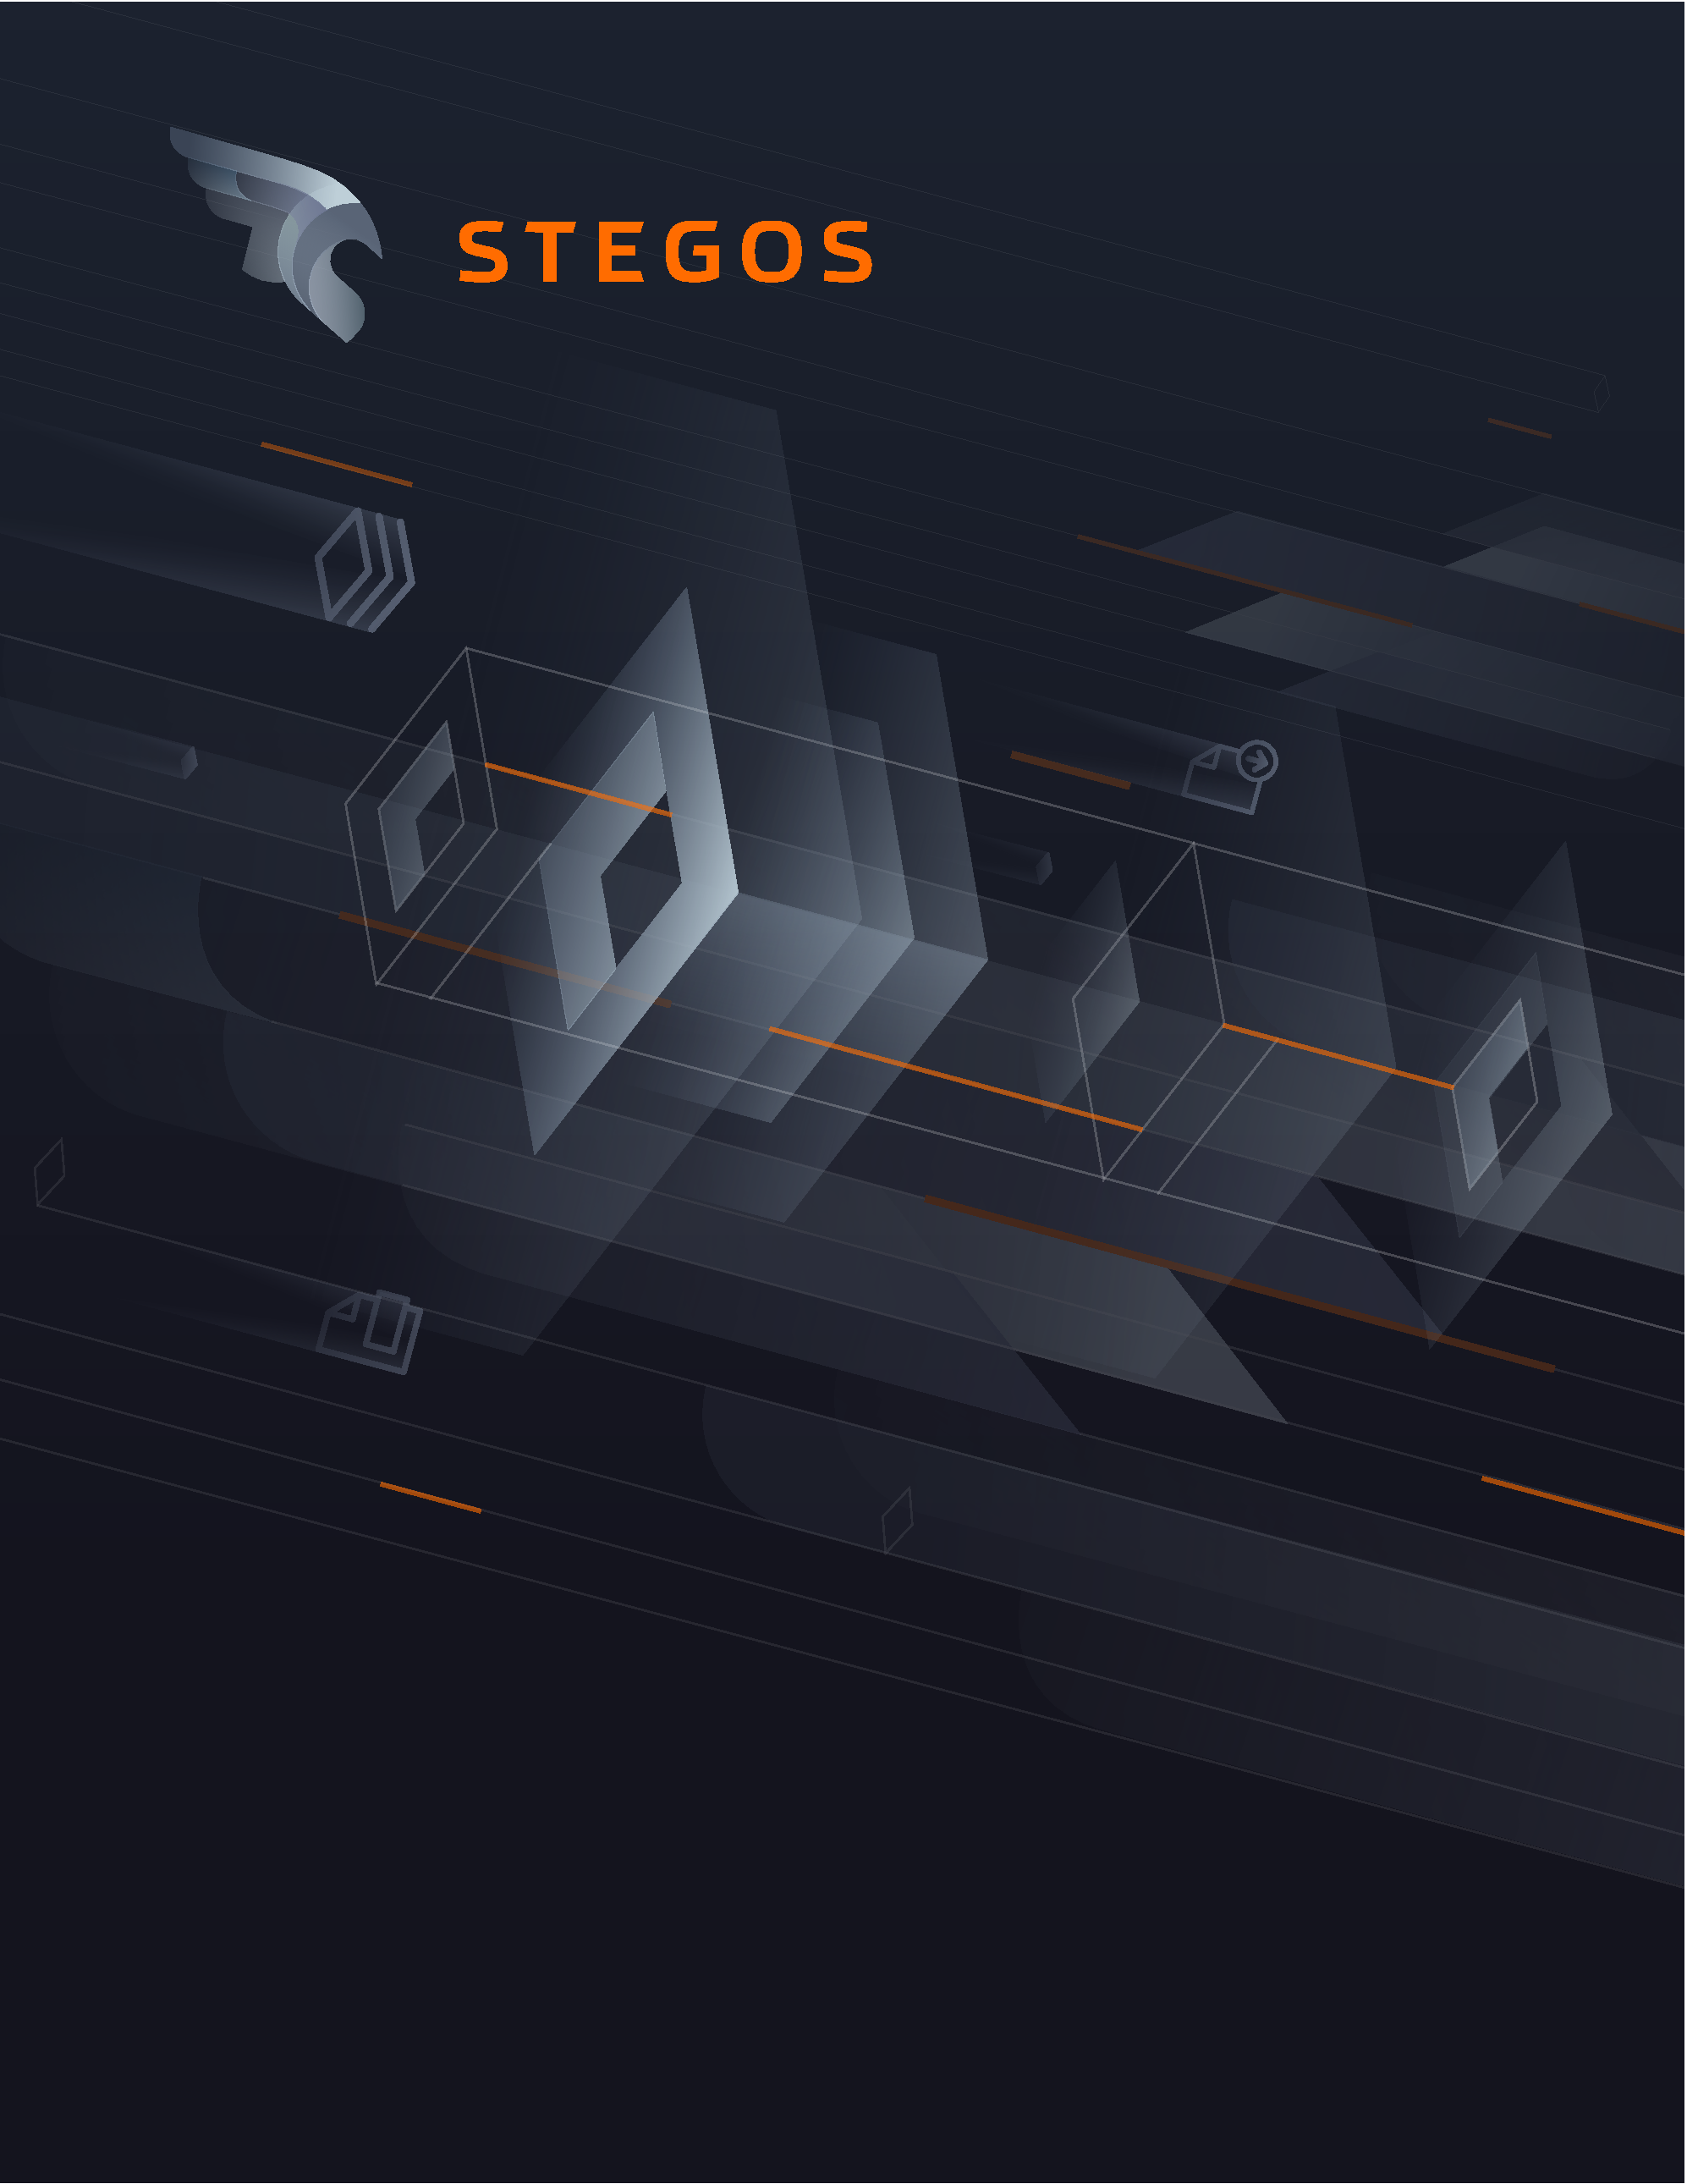
\includegraphics[width=\paperwidth,height=\paperheight]{images/front.pdf}}}
\maketitle
\endgroup

\nobreakspace

\vfill{\footnotesize\noindent{}Copyright \textcopyright\ 2019 Stegos AG\\
This work is licensed under a Creative Commons Attribution-ShareAlike 3.0
license (CC BY-SA 3.0).\\\\
All product names, logos, and brands used or cited in this document are
property of their respective owners. All company, product, and service names
used herein are for identification purposes only. Use of these names, logos,
and brands does not imply endorsement.}

\newpage

\tableofcontents\newpage

\section{摘要}
多功能移动app和社交媒体平台可以让从前无法连接起来的几百万人都能够使用在线的服务和社区。但是,他们却付出了用户隐私作为代价。相反地是,区块链和数字货币平台可以为用户带来前所未有的隐私保护,但是目前区块链技术还相对较慢,而且属于资源密集型,这就使得区块链还无法为普通用户提供服务。我们需要这种方式可以把隐私和可用性结合在单个的平台。

Stegos隐私平台(Stegos)将特殊的区块链和通证设计结合起来,并且发行了首个隐私、安全、高效以及环保的数字货币。Stegos是完全可扩展化以及不可篡改的,这就保证了区块链始终保持紧凑,而且不会损害信任。这让Stegos成为了全球首个能够提供除了支付转账之外,还有安全且隐私的数据存储和转移的公链。

Stegos将区块链底层扩展,从而提供了能够打造隐私应用的平台,并且这些应用可以为社交聊天带来最小的延迟效果。我们提出的可信应用存储(TAC)以及隐私应用商城可以让搭建和分发隐私应用的过程变得很简单,同时也能够提供更高的用户安全性。最后不能不提地是,Stegos市场、聊天、以及红包功能是去中心化应用中最流行的功能,这些可以让用户能在完全隐私地情况下进行转账和聊天。

Stegos的共识机制是赌注权益证明(gPoS)共识机制,它是基于可验证的无偏分布随机性。gPoS机制可以让任何人随身运行Stegos区块链,并且通过维护网络可以赚取收益,甚至无需很高的抵押。这可以鼓励更多的人参与,从而保证移动用户有足够的激励来验证网络。
\section{反馈}

如果对于此白皮书有任何建议,请发送邮件至\href{mailto:paper@stegos.com}{paper@stegos.com}.

\chapter{介绍}\label{chap:intro}

\section{我们都应该掌握隐私}
每个人都应该掌握自己的隐私,同时也应该获得现代社会所有的服务和福利。但是现在的技术和商业模式并不能实现这点,或者说压根不愿意,同时提供这两个服务。

过去10年,我们看到的全球社交媒体平台和多功能应用的崛起,其中都会带有支付功能,例如微信和Facebook。随着移动互联网技术的快速发展,这可以让大约10亿人能够在线上进行沟通、交易以及合作。但是这些平台的隐私功能是个噩梦:你任何的行为都可以被追踪,并且拿出你和别人的聊天或者转账记录,不论你是否想要分享这些信息。同时,用户数据会被随意地盗用,从而变成了广告商和黑客的目标。目前为制止这种滥用所作的努力是徒劳无功的,而且并没有什么意义,通常是因为政府和监管机构不希望放弃控制,让用户对自己的网络行为负责。

从硬件角度来看,固态技术、智能手机以及物联网技术把生活装进了我们的口袋、手机和电脑。但是在保护我们隐私的表面下,从恐怖主义,从黑客,从我们自己所谓的缺乏责任角度来看,我们的隐私早就被严重破坏。在机场,甚至在街上,我们被迫以惊人的频率泄露我们的私人数据。

这种入侵让我们感到隐私暴露在空气中,并且十分无助。很多人都面临着更加令人毛骨悚然的结果,例如失去工作、自由甚至生命。

我们生活在一个史无前例的国家监视和镇压新闻自由甚至思想自由的时代。但是,其实你如何对待自己的资金,无论是现金还是数字货币,又或者是如何通过区块链去进行交易,这都和别人无关。

这个趋势并没有被忽视。纵观世界上各个国家,人们对他们的隐私和数据是如何被利用以牟利表示不满。因此,我们需要更加安全和隐私的选择,而且这只会在未来几个月以及几年里持续增长。

\section{区块链和隐私}
从另一个角度来看,区块链和去中心化技术促进了数字隐私和安全领域的巨大飞跃。虽然传统的数据分享和存储技术(在线云存储,邮件,笔记本电脑等等)已经有了内置的安全性,但是这些技术很容易被攻破。一旦有人获得你的密码,并且进入你的系统,那么你的数据就会永久暴露。

基于区块链的私有的去中心化解决方案会更好地保护你的私人信息,并且可以和你信任的人进行共享。

但是,大众对于这种解决方案的接受程度却不是很乐观。目前的区块链运行速度很慢,运转不够流畅,而且对环境也有影响,而且没有任何隐私币真正地拥有它所说的隐私性能。对于资源匮乏的静态硬件以及不友好接口的依赖,最终会让这项技术远离普通用户,但是如果没有用户的参与,区块链平台注定会萎缩和重新变得中心化。随着用户的使用习惯从桌面端到移动端,加密货币其实很难跟得上这个潮流。

解决方案很清晰:为了跟上这个潮流,区块链平台必须学习例如微信和Facebook这些平台的吸引力和可用性,同时还要保持很强的隐私性、匿名性以及去中心化。

Stegos是首个将这些领域结合起来的区块链。Stegos是为安全转账、数据转移以及通信的最好机制,因为和传统的邮件和在线通信服务于不同,它是完全去中心化的、加密安全的、同时也不会留下用户身份的蛛丝马迹。因此,不会有人能看到你给谁发送信息或者接收了谁的信息,又或者确定任何人和Stegos建立联系。只有信息或者交易的接受者会知道发送的具体金额,而且没有任何东西可以将数据或交易与任何人的真实身份联系起来。

Stegos同时也是首个适配于移动设备的区块链:智能手机节点可以有完全的验证能力,并且无需基于硬件的工作量证明,这意味着任何人都可以通过支持Stegos网络获得代币收益。通过把数据转移和信息通信作为和转账相同的优先级,Stegos会是所有人都想使用的区块链。而且,专注于移动手机意味着所有人都可以使用。

在我们现代社会,每个人都应该有安全和隐私的交易和通信。Stegos是首个并且仅有的区块链平台,能够提供这些功能。

\chapter{Stegos是什么?}\label{chap:what-is-stegos}

\section{简介}
Stegos隐私平台(Stegos)将独特的区块链和通证设计结合,并且发行了首个完全隐私、安全、高效以及可持续环保的加密货币。Stegos使用了\textit{UTXO} (代币)模型以及\textit{gPoS} (赌注权益证明)共识机制,将现有的隐私代币和最新的加密研究结合,从而创建完全的可拓展(scalable)以及可修剪(prunable)的隐私区块链和应用平台。

\subsection{绝对的隐私}
由于Stegos中的雪球协议(Snowball protocol)(请见附件\ref{app:snowball}),Stegos中的支付和数据转账是不可链接的、不可追踪的、并且完全隐私的。每个Stegos中的交易是跳转到全新的、独特的秘密地址,从而无法发现接受者。雪球同时也让追踪Stegos交易历史变为不可能,因为单个交易首先会集合起来,才能在提交给区块验证者之前,形成超级转账(supertransaction)。所有这些都会通过安全、隐私保护的方式进行,同时确保Stegos代币是完全可替代。

\subsection{支付和信息传递}
其他隐私类代币 - 例如Monero, Dash, ZCash和Grin - 只可以用于支付,而且对于可扩展性、隐私性、安全性或者可用性来说,都存在缺陷。Stegos就这些和其他隐私币的问题进行了提升和优化,同时可以用于支付和数据的发送,并且是完全隐私的。Stegos可信的应用存储器(TAC)可以让开发者很容易地搭建应用,并且能够匿名、隐私并且高效地进行沟通。

\subsection{可扩容性和数据压缩}
Stegos是一个快速并且高度扩容的区块链,而且和其他区块链不同,它在不损失信任的前提下,整体保持较小。花费代币和数据消耗的细节都可以通过安全加密修剪的方式,从区块链上安全移除。由于交易分片机制,Stegos区块链具有很高的扩容性,这就让其成为世界上首个能够提供除了交易转账以外,还有安全以及隐私数据存储和传输的公链,这也让Stegos可以在智能手机上运行。

\subsection{权益证明(PoS)}
Stegos是环保的,并且不会浪费电能去挖矿的区块链。相反,Stegos使用了定制化的赌注权益证明(gPoS)机制,这是基于分布式系统理论和加密学的进步。每个Stegos区块必须由一群验证者(validators)进行验证和确认,所有的验证者必须要将代币作为抵押。通过这种方式,抵押代币的价值直接影响了验证者挖出区块,并且获得相关转账费用的可能性。

\subsection{移动应用}
为了体现平台的实力,Stegos正在开发自己的原生多功能移动应用软件,并且将钱包、点对点以及群聊、应用存储器(TAC)、隐私应用商城以及Stegos红包功能整合。这个应用将会是用户使用Stegos隐私平台的网关。
	
%% Overview

\section{默认隐私保护}
最初的比特币白皮书只包含了很少部分的隐私相关内容,它假设尽管交易数量是公开的,但是也不可能将这些交易和任何真实的身份链接起来。这个假设已经被研究者、区块链研究公司以及黑客多次证明是错误的。例如ChainAnalysis这类软件已经进行了交易分析,可以让任何人很快地发现比特币和其他加密货币使用者的身份。

大多数区块链项目都跟随了比特币的脚步,进行了完全透明的设计,并且包含了可见的地址和交易数量,其中也包含了任何钱包的余额、发送和收到了多少资金、以及每个接受和发送者的地址。但是所有这些信息都成为了黑客可见的目标。随着类似防弹(Bulletproofs)协议和零知识证明(zk-SNARKs)技术的发展,我们再也没有理由去延续比特币的错误。区块链默认就应该是具有隐私功能。
	
为了达到这个目标,Stegos中的交易所是\textit{非链接的}, \textit{不可追踪的}, and \textit{保密的}:

\begin{itemize}
	\item Stegos使用一次性支付地址,从而无法去认证交易的接收方。我们的一次性地址和Monero和ZCash的隐藏地址很相似。
	\item Stegos将个人的交易整合形成超级转账,从而无法追踪交易记录。为了这个目的,我们已经开发了增强版的ValueShuffle协议\cite{c7},这是首个与保密交易兼容的代币混合协议。
	\item Stegos中的转账金额都是通过佩德森承诺\cite{c8}以及Bulletproofs范围证明(range proofs)\cite{c4}进行保密。验证者的抵押和交易费用除外,因为对于区块验证而言,这是必须要可见的。\end{itemize}

我们称这种隐私功能的组合为雪球(如果想了解更多细节信息,请查看附件\ref{app:snowball})。

\section{赌注权益证明(gPoS) 共识机制}

标准的权益证明共识让很多持有小额抵押代币的用户感受不到激励。为了解决这个问题,Stegos使用了\textit{赌注权益证明} (gPoS),其中每个验证者在运行了一段时间后都有几率获得随机的\textit{验证者服务奖励},并且这无论他们抵押代币的数量。

\footnotetext{名义上的最小阈值将让用户无法使用系统,但是因为每个可用节点必须要提供验证服务来进行认证,从而不可能去对系统进行欺诈,因为\textit{验证节点服务奖励}的目标之一,就是能够最大化不同节点的数量。}

为了提供资金,每个区块奖励的一部分会加入到服务奖励池,这个资金池会逐渐增加,直到有人赢得基于可验证分布随机性的\textit{加密彩票}。

因为智能手机节点可以有完全的验证功能,任何人都能随身赢得代币奖励。

\section{分片获得扩容性}
Stegos使用交易型\textit{分片}来进行扩容。不同的Stegos验证者会保持整体区块链的状态,但是只会验证即将进行的交易,并且使用跨分片的原子提交(atomic commits),从而消除了双花的可能性。这种扩容的方式可以让Stegos能够每秒在数百万个移动设备中处理几千笔交易,让Stegos成为首个,并且是仅有能够整体在移动端运行的区块链系统。

\section{修剪和数据压缩}
很多项目自称可以达到成百上千或者甚至几百万的每秒转账数额(tps),但是很多有项目解释它们计划如何去维护这些累积的数据。比特币区块链虽然只有7-10的tps,但是现在数据已经大于200千兆字节。假设比特币突然可以支持16,000tps,那么比特币区块链的数据会每天增长350千兆字节\footnote{https://hackernoon.com/if-we-lived-in-a-bitcoin-future-how-big-would-the-blockchain-have-to-be-bd07b282416f},也就是说每年增长127百万兆字节。如果不通过几个超级计算机,这个量级的数据是完全不可持续的,但是这和区块链的去中心化理念是相反的。

Stegos是\textit{可压缩}的区块链。通过安全的加密修剪(pruning)功能,消费的代币和过期的数据可以安全地从区块链上移除。为了让消费过的代币信息可以从区块链上移除,我们使用了中本聪在最初比特币白皮书\cite{c1}上提到的技术。数据可以自动和快速地被移除。

\section{快速数据传输}
和其他区块链不同,Stegos不会限制用户只可以进行支付。Stegos支持数据传输,可以让用户的数据传输获得和支付同样的安全性。数据是Stegos区块链中的头等公民,这是合乎逻辑的,因为一般来说,用户发送数据消息的频率比支付要多的多。

\section{Stegos移动应用}
Stegos移动应用是Stegos生态系统中的一部分,并且是我们平台潜力的展现。这个应用会整合在钱包中,并且这个钱包拥有安全的环境可以运行隐私应用。通过这种方式,Stegos能够提供现在中心化多功能应用的所有功能,例如微信等等,但是却是通过完全隐私和去中心化的方式。

Stegos快速信息传输功能包含点对点聊天和群聊,同时还有支付和红包功能。在微信中,红包功能非常著名,它可以让任何人给个人或者群聊中发红包,或者创建定制化的代币空投,从而任何人都可以扫描二维码去领取。

Stegos应用同时也可以让用户简单且直接地控制自己的抵押代币,让所有人都可以简单地参与到网络维护中来。

每个人都应该有隐私,而且每个人都应该因为贡献了更加隐私的世界而获得奖励。Stegos不仅只让你的财产和隐私安全,而且会因为你支持网络建设而给你奖励,甚至你可以使用手机来进行参与。

\section{隐私应用}
Stegos致力于满足人们逐渐增长的隐私需求,而且不会牺牲可用性或者可访问性。研究显示数百万用户都对现有的例如Facebook和微信平台不满意,但是却没有很好的替代方案可以让用户去选择。为了满足这个需求,Stegos的设计可以满足隐私应用的爆发,通过Stegos聊天,用户的聊天内容会很安全且隐私。      

\subsection{可信应用容器(TAC)}
可用性和可访问性不仅是用户的需求。开发者如果想要去新平台进行开发,也很关注这方面。开发原生的移动应用很困难,并且很容易出错,而且开发安全移动应用也很难,区块链的介入会让整体更加困难。Stegos的目标使开发移动隐私应用程序变得简单和低门槛,同时保护用户免受恶意或写得不好的应用程序的侵害。

Stegos \textit{可信应用容器} (TAC)是一个原生的移动应用和一个部署隐私应用的容器。这些应用可以通过类似Javascript、HTML以及CSS这样的技术来完成,并且可以按照类似\textit{沙盒}中的插件这样运行,拥有对用户钱包和外部环境的严格控制。

\subsection{应用商城} 
用户需要能够简单寻找和安装应用的方式。Stegos隐私应用商城会提供链上寻找和安装隐私应用的机制,并且在TAC中开发和运行,同时也可以评估它们的可用性。

\section{私人市场}
私人转账不仅是限于代币支付。虽然代币转账对于很多用户来说是非常重要的(例如汇款),大多数交易包含了对某几种商品或者服务的支付。通过将私人支付、快速信息传输、聊天以及TAC进行整合,Stegos会开发私人交易市场,其中很多东西都能够匿名和隐私地进行售卖。

Stegos会发布一个单独的移动软件作为这个市场的界面。

\section{提高应用的激励方式}
去中心化网络可以从用户中获得巨大的力量。因此,为了激励大规模应用,Stegos会包含各种激励措施,旨在吸引各类不同的用户群体。

除了标准的抵押支付会按他们的抵押比例奖励验证者,\textit{验证者服务奖励}是独特的Stegos功能,会因为验证者保持在线并且支持网络就给予他们奖励。每个区块奖励的1/3会加入到服务奖励池中,\footnote{以及那些红包过期未使用的代币.}然后会每几千个区块就进行分发。验证者会运行基于可验证分布随机性的\textit{加密彩票} ,从而选择单个验证者来获得奖励。所有用户通过Stegos应用都可以看到当前的服务奖池数量。

\textit{红包}\footnote{https://en.m.wikipedia.org/wiki/Red\_envelope\#Digital\_red\_envelopes} 是非常有名的微信功能,这也是基于中文“红包”。红包功能的引入会让几百万用户加入微信,同时他们还需要交出自己的银行卡信息。Stegos想要在不侵犯用户隐私的前提下,复制这个非常著名的功能。

正如微信中红包功能那样,Stegos红包会有不同的选项:可以是公开的,也可以是私下的,而且红包数额可以是固定或者随机的。最简单的方式,红包可以通过Stegos聊天功能,发送固定数量的代币给别人,或者是给群聊,其中的代币数量是未知的,只有你打开红包才会知道。

私聊群的红包同样可以是随机的,群里每个人都会获得随机的数额。

Stegos同时也会让用户在Stegos隐私平台内的Stegos本身、单个的隐私应用和私人市场中创建公开的红包,这个功能可以让用户传播代币,并且提高知名度。公开红包和空投类似,但是可以鼓励更多用户积极参与。

任何人可以创建公开红包,并且放入一定数量的代币。然后,他们需要将相应的二维码或者URL链接发送给目标人群,每次打开红包都会获得一定数量的代币奖励,直到红包被领完或者经过一天后,这时候所有没有领取的代币会添加到验证者服务奖励池。

关于使用Stegos红包的部署信息,请查看\ref{sec:red-packets}部分。

\chapter{隐私应用平台}\label{chap:privacy-app-platform}
Stegos隐私平台会基于我们的快速信息传输功能(Section \ref{sec:fastdata}),并且使得开发移动隐私拥有变得非常容易。Stegos移动应用是整个平台的窗口,它会将可信应用存储器(TAC)和点对点以及群聊,还有隐私应用商城和红包功能整合起来。

\section{可信应用容器}\label{sec:tac}
可信应用容器(TAC)是一个沙盒和虚拟机(VM),并且可以运行通过HTML, CSS和JavaScript语言编写的内置应用。这个技术底层和微信小程序很类似 \footnote{https://walkthechat.com/wechat-mini-programs-simple-introduction/}。

TAC会防止应用程序对主机造成破坏,同时也让区块链从运行应用中完全抽象出来,而不是提供接口(API)来发送信息并且进入钱包。TAC严格控制对外部世界的访问,并确保消费代币需要用户确认。

Stegos会提供搭建隐私应用的软件开发包(SDK)以及相关文件。

\section{身份信息}\label{sec:identity}
每个Stegos钱包都带有公钥(地址)。Stegos使用\textit{隐藏地址},从而对公钥的支付被两个随机值掩盖,这样就无法通过分析区块链去发现转账人的身份。只有发送方和接收方才有权进行任何信息交换。这意味着用户不必太过保护自己的公钥:将Stegos公钥发布在网站或者甚至把它贴在街上的广告牌上,这都是完全安全的。

Stegos使用了未花费交易(UTXO)模型,其中每个UTXO都可以理解为一个代币。在Stegos中,没有任何单独的身份概念,尽管钱包地址可以用作标识符或化身,用于发送信息或在Stegos私人市场或其他隐私应用程序上建立声誉或社会评分。

Stegos用户能够将钱包地址导出作为二维码。

\section{隐私应用商城}\label{sec:appstore}
用户有着不同的隐私需求,有时候甚至用户下载的app都会面临隐私泄露风险。用户需要有隐私地浏览和进入app应用的方式,虽然他们认为自己下载和安装的app是隐私和安全的。为了达成这个目标,Stegos部署了链上隐私app商场,其中这些应用的细节都存储在Stegos区块链上。

这些app本身应该是链下存储,并且不会影响到Stegos区块链,而且需要上线Stegos隐私应用商城,每个隐私应用都必须创建声明,其中包括app的描述,下载URL链接,以及应用程序包的哈希,这个声明会存储在Stegos区块链上。App中包含了标签,可以让用户通过类别在app商城里面搜索。

App会通过Stegos商城下载,一旦下载成功,TAC会验证应用程序包的签名,以及哈希是否符合声明中的信息。TAC会在本地安装应用程序包,并且让这个应用在Stegos移动应用中可用。用户随时都可以删除这些应用。

\section{聊天}\label{sec:chat}
无论在这些转账中区块链是如何模糊用户信息,用户仍然需要找到对方,这就有暴露个人信息的风险,这些造成比代币更大的影响。例如,MimbleWimble需要用户提前进行通信,从而可以分享在交易过程中确定身份信息所需要的因素。但是每个交易都需要用户间的一些初始通信,从而确定交易的参数。如果这个通信能被截获,那么恶意的第三方都会开始对交易记录去匿名化。

现在的平台都会把这个问题留给用户去解决,大大降低了它们的吸引力和有效性。虽然这些信息泄露无法完全满足,但是在Stegos平台,我们相信这是我们的责任去给用户尽可能多的工具去保护他们的隐私。每个能通过这种方式保护的平台都会提高平台用户的隐私性能。

最终,Stegos会部署完全私人的通信,并且将其和Stegos应用整合,它会包含类似标准通信应用,其中所有用户都对它很熟悉。用户使用公钥作为身份认证(Section \ref{sec:identity}),在不泄露任何与其他用户交易信息的情况下展示出来。信息会通过快速信息总线(Section \ref{sec:fastdata})进行传递,从而确保信息是几乎即时收到。

用户可以通过私聊发送二维码,从而启动STG转账,同时也可能创建聊天群,并且通过二维码邀请用户进群。

接下来的章节,我会更详细地介绍Stegos功能。

\chapter{Stegos详细解读}\label{chap:stegos-in-depth}

\section{共识机制}
Stegos共识协议是基于\textit{Albatross}\cite{c23},这是通过拜占庭机制BFT\cite{c9}的全新区块链共识算法,而且在获得及时交易确认的同时,还有很强的一致性。Stegos共识协议是安全的,并且和理论上获得单链PoS共识机制的最大值。

\subsection{投机拜占庭容错}
投机拜占庭容错(SBFT)算法有两种共识模式:

\begin{enumerate}
	\item the \textit{乐观模式}, 转账速度很完美,但是只有很少的安全错输,假设所有的节点都运行良好。 
	\item the \textit{悲观模式}, 唯一的目标是在有欺诈节点的情况下,系统也能顺利运行。 
\end{enumerate}

乐观模式可以让Stegos共识协议能够和中心化系统类似的速度。节点会验证每次状态更新,当有无效更新检测出来的时候,共识就会切换到悲观模式。无效的更新就会被丢弃,然后共识回到乐观模式。

\subsection{验证节点}
Stegos是公开账本,因此每个人都可以加入网络,成为验证节点,同时通过维护区块链获得奖励。和标准的PoS共识相比,Stegos使用赌注权益证明(gPoS)共识来更好地激励散户参与。节点需要进行绩效绑定(抵押),从而可以进行验证服务。通过给出经济方面的抵押,要求验证节点都提供绩效绑定,从而防止女巫攻击。锁定的代币可以像普通代币那样进行权益抵押。

给出绩效绑定的验证节点能够被随机选择,去作为活跃验证节点参与确定共识。每个活跃的验证节点都会通过可验证的分布式随机方法去创建区块,同时还会从交易手续费中获得奖励。其他活跃验证节点会见证并且同时签署创建的区块,从而可以获得验证节点服务奖励(Section \ref{sec:service-award})。

\subsection{区块}\label{sec:blocks}
Stegos有两种类似的区块:

\begin{itemize}
	\item {\em 核心区块} 核心区块是用来改变验证节点列表,并且作为Stegos区块链上的检查点。核心区块只包含了活跃验证节点的身份信息,以及用来选择它们的随机助记词。核心区块是通过实用性拜占庭证明(pBFT)产出,并且不会分叉。
	\item {\em 普通区块} 每个普通区块都是通过可验证的随机方式选择出的活跃验证节点产出,并且不仅包含了用户转账信息,还有目前的状态以及验证节点的随机助记词。这些区块是通过乐观方式产出,并且只需要相应的验证节点签名。
\end{itemize}

一个核心区块总是带有固定数量的普通区块。一个\textit{epoch}是由一个核心区块和相应的普通区块组成。每个epoch中,验证者列表会更新,并且全新的活跃验证节点会随机选出。

\subsubsection{区块生产频率}
在测试环境下,假设$16$-节点的网络,我们观察区块传播的时间为$500ms$ - $700ms$。实际运行中,时间可能会更长,但是对于普通区块来说,速度也会在$5s$之内。

核心区块包含了实用性拜占庭共识(pBFT),因此会需要更长时间来进行创建。测试过程中,我们观察到对于$16$ 验证节点来说,其时间大约为$5s$。验证节点的数量在实际过程中会更多,但是我们认为区块生产频率会在$30s$到$60s$。

核心区块生产时间$2min$应该可以保证核心和普通节点的比例足够,从而在不损失安全性的情况下,可以去应用乐观模型。

\subsection{验证节点选择}
验证节点通过权益加权彩票的方式从验证者池中选出。随着验证节点抵押的金额越大,在创建核心区块的时候,它们就有更高的概率可以成为实用性拜占庭证明(pBFT)的领导者,或者被选择成为创建普通区块的所有者。

\subsection{消除分叉}
验证节点只会选择最长的区块链,也就是说有着最多区块的链,称为主链。因为核心区块需要pBFT共识,分叉只可能在两个核心区块之间进行。因此,节点只需要专注于考虑包含最新核心节点的区块链。

我们通过从上到下的启发式算法来解决分叉:

\begin{enumerate}
	\item 有着最多核心区块的区块链。
	\item 有着最高pBFT视图更换区块的区块链。
	\item 有着最多区块的区块链。
\end{enumerate}

在所有这三个条件下都发生的情况下,下个验证节点可以基于其他链继续搭建。

\subsection{惩罚恶意节点}
在我们的共识机制下,恶意节点有三种方式:产生无效区块、创建分叉以及延迟区块。这些需要将在适当的情况下予以处理和抑制。

我们通过以下方法处理这些恶意行为:

\begin{enumerate}
	\item {\em 无效区块} - 当验证节点产生了无效区块,其他验证节点会无视这个区块。验证节点同时会忽视从这个验证节点中输出的其他区块,这样可以防止DoS攻击。
	\item {\em 分叉} - 在核心区块中,分叉是不可能的,因为pBFT共识是无法分叉的协议。但是如果验证节点同时产生了超过一个普通区块,那么分叉就会产生。这种情况下,分叉会被忽视,并且一个新的活跃验证节点会通过pBFT视觉转换协议选出新的活跃验证节点。 
	\item {\em 延迟} - 验证节点可能导致产生区块的时间过长,或者完全掉线。这两种情况下,我们会通过pBFT视觉转换协议改变这个位置的拥有者。 
\end{enumerate}

为了抑制这些行为,我们引入了\textit{削减}来惩罚那些恶意的验证节点。削减(slashing)方式会没收那些验证节点的抵押代币,如果他们产生了无效的区块或者分叉。证明分叉的唯一证据是两个区块头部由相同的验证节点签名,而被没收的抵押代币会平均分发到目前epoch中剩余的验证节点。区块延迟不会通过削减方式进行惩罚,因为无法知道这个延时是否是恶意欺诈,而且我们不想去影响移动节点的积极性,他们更可能有不稳定的网络连接。

\subsection{集体签名}
我们使用了\textit{CoSi}\cite{c10,c11},这是可扩展的可见证共同签名协议,从而确保每个授权的状态是有效的,并且在客户端接受结果之前,由不同群体验证者公开记录。状态$S$是由$W$个见证者集体签名,从而确保$S$被$W$ 见证,并且不会立刻发现错误。

如果$S$没有被见证者检测出来,CoSi也会保证$S$接受公众监督,从而让攻击者冒着很快就被$W$见证者发现的风险。

Cosi基于现在的加密多重签名方式,并且将它们通过高效通信进行签名聚合,从而能支撑数千个见证者。Cosi的默认部署是Schorr签名,但是因为效率原因,我们替换为BLS签名。

参与Cosi的活跃见证节点可以获得验证解决服务奖励(Section \ref{sec:service-award})。

\section{网络}
Stegos网络是由三个类型的节点组成:\textit{引导节点}、\textit{压缩节点}以及\textit{轻钱包}。引导和压缩节点会维护区块链以及相关数据结构的复制版本。在发布绩效绑定(抵押)从而成为\textit{验证节点}后,这些节点会参与到共识协议中,并且能够获得区块奖励以及转账费用。这些节点也会回应轻钱包节点的需求。

引导节点会承载未修剪的区块链版本,并且从全新的压缩和引导节点中回应引导需求。压缩节点会承载修剪完成的区块链版本,也就是说,目前的UTXO设置。轻节点只会保留区块头部,以及了解如何和验证节点进行交互。

Stegos初始会通过运行几个核心引导节点去维护核心网络,从而保证网络的可持续性和性能。这些核心节点的地址会硬编码到Stegos区块链软件的每个发布版本。

节点会保留地址列表,并且将其他客户端添加到地址上,从而让他们直接互相知晓。新节点会和其中一个核心节点连接,从而获得引导节点列表,然后下载区块链副本。

经过一些轻检验,每个全节点都会很快地重新播放获得的转账给其他客户端。这就保证了节点不会因为有大量垃圾交易而受到DDoS攻击。为了抑制不良行为,我们引用了一种机制去防止客户端作恶,并且会对恶意转账进行惩罚,例如,让他们后续无法参与网络。

Stegos区块链使用了Gossip协议来传播信息,而且不用依赖于固定的网络结构。这个协议无需每个节点都可靠,或者总是在线以及运行,而且无需每个节点都互相知晓。每个节点都仅知道几个客户端,而且信息也可以安全地通过网络进行传播,主要大多数节点知道至少2个客户端。

\section{激励措施}
Stegos是由STG代币赋能的,在主网上线的时候,STG代币就会可用.当节点进行抵押并且希望支持Stegos平台的时候,当他们被选为共识阶段的领导者,则会获得STG代币作为手续费以及区块奖励.验证节点选为领导者的可能性是和他们持有的代币成正比.

\subsection{验证节点服务奖励}\label{sec:service-award}
基于权益证明(PoS)的账本很难去维护一个很广的用户基数,因为大多数用户都只有很小的几率去赢得很大的奖励。为了弥补这点,gPoS协议除了标准的区块奖励和交易手续费,还包含了\textit{验证节点服务奖励}。这些奖励是为了那些抵押金额较小的验证节点,去维护网络安全。除了只把奖励分发给区块创建者,任何有活跃验证服务的节点都可以赢得奖励。这可以增加对普通区块激励见证以及核心区块参与到pBFT过程的效果。

每个区块奖励的1/3都添加到服务奖励池中,同时还有过期的红包奖励。验证节点服务奖励是奖励给单个用户的,这样用户是所有从上个验证节点奖励服务支付给出后,已经提供验证服务的用户选择。奖励一开始比较少,但是会随着区块而增加。因此无法预测精确时间,但是平均来说,验证服务奖励会在每5-10天进行分发。选择频率是为了保证提供抵押的最多用户可以有机会成为节点,而且奖励应该总是足够多,才能成为吸引更多人参与的激励。

\subsection{红包}\label{sec:red-packets}
捐赠是最受欢迎和有效的方式,去提高参与度和平台的知名度。因为微信电子红包2014年兴起,数以百万的人都注册了微信,并且共享了他们的银行信息。仅2016年,红包应用已经有超过20亿笔交易。

对于加密货币平台来说,最常见的形式是空投。但是这种方式的效果很差,因为空投其实很难去激励参与度,并且他们的长期效果是不清晰的。虽然空投看似对于社区成员有效,但是很少有人去运行节点或者有效地运用这个平台。

为了解决这个问题,Stegos实施了类似微信的红包功能,但是无需用户去披露身份认证。红包会以两种方式出现:私人的和公开的。私人红包可以用来发送固定数量的代币,给予特定的个人或者群聊。公开红包是随机的红包空投机制。

Stegos应用的任何人可以创建红包,并且放入STG代币。除了红包里面的代币数量,用户也会选择奖品的数量(如果是给特定用户,那么红包数量就是1)。那么,这些代币就会随机分配在红包中的不同UTXO中,并且代币的数量和选择奖品的数量相等。

然后,这个应用会产生二维码或者URL链接,这可以用于进入红包。进入红包后,验证节点会随机决定用户是否会获得奖励。如果他们有奖励,其中的代币就会从钱包转移到用户的STG钱包。这个过程会一直持续直到红包空了或者过期。

用户可以一直抢红包直到空掉,但是网络会有微弱的延迟从而防止DDoS攻击。抢红包是免费的,而且无需用户购买代币或者支付交易费用。但是,所有奖励中的一部分将会作为手续费奖励给验证节点

红包会在一天后过期。由于Stegos交易的隐私属性,因此是无法退回没有领取的红包。因此,这部分红包会加入到验证者服务池。

用户必须要安装Stegos应用,并且设置STG钱包,才能打开红包。通过这种设置,用户才能通过最少的成本去运行移动验证节点。

\section{雪球}
\subsection{建立不可追踪的问题}
尽管用户身份是存储在区块链,每个UTXO交易的历史都会通过追踪区块链交易奖励获得,一直追溯到创世区块。

尽管对于这种追踪有比较严重的阻碍 - 我们不会在区块链的区块中存储交易,而是输入和输出的Merkle树- 主网发布后,立刻加入Stegos网络的欺诈节点理论上会获得所有交易记录,从而去分析并且追踪UTXO。

为了解决这个问题,Stegos会部署一个完全隐藏每个交易输入和输出关系的协议。这是很困难的,因为UTXO必须有$ID$,如果没有则无法去验证节点或者说验证UTXO的身份。特定UTXO的ID会建立一条线索,我们会可以通过展示UTXO的输出.

\subsection{可能的解决方案}
现在,可能有四种方式来解决无法追踪的问题:代币混合器、环形签名、零知识证明以及CoinJoin协议系列。

\subsubsection{混合器} 代币混合器需要用户信任提供混合服务的第三方机构,这对于完全私有化和隐秘的区块链来说,是不可接受的。

\subsubsection{环形签名} 环形签名需要收集大量随机的UTXO,然后将它们添加到实际发出的输入列表。所有这些输入会形成签名,从而让这些值通过集群的方式发出,而无需揭露真实发出的输入数据。 

不幸地是,环形签名阻碍了区块链压缩,因为不可能知道UTXO发送的时间,并且从区块链中进行修剪。所有UTXO\textit{曾经出现过的}必须保留,这就导致无法进行扩容。

\subsubsection{零知识证明} 零知识证明是“零知识简洁的非交互知识论证”的缩写。目前,产生足够短且可以发布在区块链中的零知识证明是通过初始设置去获得证明者和验证者共同分享的字符串来实现。任何能够获得用来产生这个字符串的秘密随机数的人可以创建虚假的证明,而且验证者还会认可它。对于使用零知识证明的加密货币来说,例如Zcash,这意味着能够制造假币的能力。

为了防止基于零智商证明加密货币的双花现象,节点必须持有包含很多已消费代币系列号的加密累加器。这个累加器会一直增长,并且无法修剪,这样就导致无法扩容。

\subsubsection{CoinJoin} 协议可以在提交比特币交易数给矿工之前混合几个不同的数据。这个协议最初是Greg Maxwell在2013年最先提出的,并且它的原理如下:“当你进行支付的时候,会找到其他也想进行这个支付 的人,并且同时进行支付。”\footnote{https://en.wikipedia.org/wiki/CoinJoin} CoinJoin是基于可信服务器,从而可以将多个交易数据混合,从而为系统带来相对的安全性。

每种方式都会有不可接受的手续费用后者需要相当的信任条件,而且大多数要求是无法解决的。但是,CoinJoin的方法能够解决信任问题。2014年,CoinJoin让德国萨尔州大学的研究人员开发了完全的去中心化协议,并且称为\textit{CoinShuffle}\cite{c17}。 它也让用户去互相混合自己的代币,并且使用匿名沟通协议 \textit{Dissent} 来保证匿名性,同时也能防止DoS攻击。

2016年,相同的研究人员发表了增强版的协议,他们称为\textit{CoinShuffle++}\cite{c18}。CoinShuffle++的核心创新是将混合网络替换为Dining Cryptographers Networks (DC-nets)\cite{c20},这是更为有效的匿名机制。

混合网络需要连续的运行,因此初始CoinShuffle协议的通信次数和用户数量成正比。通过使用DC-nets网络,CoinShuffle++可以让混合器同步运行,从而无论有多少用户都可以获得稳定数量的通信次数。

Stegos采用了CoinShuffle++ 功能,但是进一步提高了这项技术。

\subsection{ValueShuffle}
\textit{ValueShuffle}\cite{c19} 是CoinShuffle++的扩展,并且可以和隐私交易功能兼容。ValueShuffle确保了多个成员混合的匿名性,同时也有支付数额的隐私性,甚至还可以防止欺诈成员。Stegos应用了这个方式,同时也在几个核心区域提升和完成了这项技术。首先,ValueShuffle白皮书丢失了几个核心的细节:例如,白皮书没有提供任何关于如何形成这样系统的细节,也没有如何在交易数据进行签名的方式。

我们使用了这个协议,其中\textit{facilitator}是从验证者中选出,并且提供\textit{Bulletin Board} (根据ValueShuffle协议中的定义)服务。我们也会在结果交易数据中部署集体Schnorr签名\cite{c22}。这些协议的细节,以及ValueShuffle的细节都在附录\ref{app:snowball}中体现。

\section{BlockCrunch}\label{sec:pruning}
BlockCrunch是进行修剪区块链的Stegos算法,并且保持区块链压缩。通过在\ref{sec:blocks}章节的描述,普通Stegos区块链是由区块头部和区块主体组成,其中头部带有两个Merkle树的头部哈希,并且和区块主体兼容。这两个树是所有输入数据组成的树 (\textit{TXIN} Merkle tree),而且所有输出数据组成的树 (\textit{TXOUT} Merkle tree)。

当全新的区块进行验证和签名的时候,这个签名就会根据区块头部进行计算。区块主体无需签名,因为通过了Merkle树的天然属性造成。那也就是说,没人可以修改区块主体的内容。

Stegos区块链的压缩是个连续的过程,其中每个签名的区块都会触发修剪功能。最后,Stegos区块链就会成为UTXO数据库,并且没有存储任何交易历史数据。

完成验证和签名新区块后,\textit{leader} 会将这个记过播放到网络。所有节点必须验证整合的区块签名,并且通过以下步骤处理新区块:

节点必须为任何普通区块进行下面的修剪算法:

\begin{algorithm}
\begin{algorithmic}
	\State $block \gets <This Block>$
	\State $tree \gets \Call{Get-TXIN-Merkle-Tree}{block}$
	\State $leaves \gets \Call{Merkle-Tree-Leaves}{tree}$
	\For{$leaf \gets leaves$}
	\State $id \gets \Call{UTXO-ID}{leaf}$
	\State $block’ \gets \Call{Find-Block-With}{id}$
	\State $tree’ \gets \Call{Get-TXOUT-Merkle-Tree}{block’}$
	\State $leaf’ \gets \Call{Find-Leaf}{tree’, id}$
	\State \Call{Mark-As-Spent}{$leaf’$} \Comment{Does not touch the hash of the leaf}
	\For {$sibling \gets \Call{Get-Sibling}{leaf’}, \Call{Is-Spent}{sibling$}}
		\State $parent \gets \Call{Get-Parent}{leaf’}$
		\State \Call{Mark-As-Spent}{$parent$}
		\State \Call{Delete-Node}{$leaf’$} \Comment{Removes the hash}
		\State \Call{Delete-Node}{$sibling$}
		\State $leaf’ \gets parent$
	\EndFor
\EndFor
	
\If {$\Call{Is-Empty}{tree}$}
	\State $\Call{Delete-Tree}{block, tree}$ \Comment{Leaves just the hash in the block header}
\EndIf
		
\end{algorithmic}
\caption{Pruning algorithm}
\label{code:pruning}
\end{algorithm}

\section{快速发送数据}\label{sec:fastdata}
Stegos在普通支付交易之外,还增加了数据传输功能。这两者都有相同的加密性和隐私保护。其实,由于这些数据是通过无价值代币发送,无法将支付和数据信息分开。

数据信息会在不同的应用层,并且有效负载应包括序列号。和支付不同,数据不会有双花,因此无需等待数据信息变为不可逆。信息序列号应该帮助应用获得信息,并且可以检查丢失的信息。

Stegos数据信息非常像UDP/IP,并且可以作为任何应用能够安全和隐私地进行沟通的信息通道。

数据信息会自动循环,并且通过BlockCrunch (Appendix \ref{sec:pruning})从区块链移除。

\chapter{未来的工作}\label{chap:future-work}

\section{移动端抵押}\label{sec:mobile-staking}
主网上线的时候,移动端抵押不会开通。但是,我们会尽快启动,移动端代币抵押会大幅增加验证节点的数量,提高网络的稳定性和吞吐量。和ePoS相比,这会防止很多区块链项目都面临的拥堵和中心化问题。

\section{交易市场}\label{sec:marketplaces}
完全的隐私代币转账是非常有用的,但它们本身只为私人交易提供必要功能的一部分,其中大部分涉及商品和服务的交换。只有在交易的其余业务不能被混淆的情况下,才能私下转让代币。目前,大多数隐私平台都将这个问题留给用户来解决,从而大大降低了它们的可用性。

通过搭建这些功能,Stegos隐私交易市场可以提供售卖产品和服务的必要工具,甚至可以将整个市场都进行完全的隐私。

商户可以在TAC中设置微店,并且使用钱包公钥作为身份认证。API可以让商户更新库存,通过隐私应用(Section \ref{sec:appstore}),用户可以浏览特定的商店,并且通过商户的公钥签名来进行认证。用户可以通过特定的市场应用进入Stegos市场,买卖者可以通过Stegos聊天服务进行沟通(Section \ref{sec:chat}).。

私有市场使用了hashlock(TBD)的方式来自动完成支付,并且只有交易双方都满意条款,支付才能完成。

\subsection{信誉系统}
线上市场通常会依赖于排名和信誉系统,从而让购买者可以通过将评价和评级上传至区块链而完成这个功能,同时会用公钥进行签名。当通过市场应用去搜索商户的时候,评价和评级会记录在链上,从而让买家能看到每个商户认证后的整体评级。

不幸地是,任何将这些交易连接起来的东西都会存在潜在的隐私风险,因此用户必须根据自己的隐私需求去权衡。因此,是否加入评级系统是商户可以自由选择的。

\section{路线图}\label{sec:roadmap}

\begin{table}[ht]
\centering
	\begin{tabular}{@{\extracolsep{4pt}}lll}
	\toprule[2pt] 
	年份 & 目标日期 & 可交付产品 \\
	\midrule[2pt]
	2019 & 31.05 & 主网以及原生代币\\
	{} & {} & 跨平台节点 UI \& 钱包 \\
	{} & Q3 & 交易所代币销售 \\
	{} & {} & 移动端 app \\
	{} & {} & 蒲公英协议 \\
	{} & Q4 & 分片 \\
	{} & {} & 移动 (压缩) 节点 \\
	{} & {} & 移动端抵押 \\
	2020 & Q1 & 应用商城 \\
	{} & {} & 私人交易市场 \\
	{} & Q2 & 无引导节点的区块修剪功能 \\
	{} & {} & 零知识证明 \\
	\bottomrule[2pt]
	\end{tabular}
\caption{Roadmap} 
\end{table}

Stegos团队目前正在部署区块链技术,并且开发进程可以通过\href{https://github.com/orgs/stegos/projects/1}{GitHub}进行追踪,我们平台的代码是100\%开源。

\section{结论}
此白皮书解释了Stegos\textemdash 是如何设计一个隐私的、保密的以及稳定的区块链体系,并且它对环境也友好,能够优化数据和支付存储以及转移功能。

其他隐私项目都会对隐私做妥协:需要用户接受速度更慢,并且更加消耗能源的区块链,从而获得可能的隐私提升。他们对于信息转移也没有很深入的思考,让用户学会如何私下沟通和协调他们的交易条款。

Stegos是不同的,它结合了最先进的隐私技术以及更快更具扩展性的区块链 \textemdash ,同时还有足够的创新 \textemdash 从而创建让带有隐私性能的区块链更加高效,而不是变得低效。

通过对区块链进行修剪,Stegos能够支持很多不同的链上功能,而不只是代币转账。通过将聊天、在线应用商城以及可信区块链容器(TAC)等结合,Stegos推动了产品和服务的完全隐私化交易,而不仅是最后的支付功能。

Stegos使用了可验证的随机数,以及赌注权益证明机制去创建首个可信任的移动区块链体系。通过整合手机,并且提供整合app应用作为平台的网关,Stegos旨在成为首个可应用的区块链平台,让任何人都可以获得他们所应得的隐私性。   

\chapter{团队成员}\label{app:team}

Stegos团队不只是有区块链经验(虽然我们的技术实力也很强)。我们团队有着金融、飞机以及加密学方面的经验,该团队在将技术应用于社会面临的一些最敏感的挑战方面拥有广泛的经验。

\section{Joel Reymont CEO, 一切我负责!}

{
\setlength\intextsep{0pt}
\begin{wrapfigure}{l}{0pt}
	
\includegraphics{images/team/team-1.png}
\end{wrapfigure}

Joel是经验丰富的黑客和区块链先驱。他在华尔街开始了自己的事业,并且将25年的软件工程和管理的经验带入了Stegos项目。Joel之前是市值前100加密货币和区块链公司的首席技术官,而且他在社区也获得了很好的声誉。Joel是德意志银行首席经济技术总监,管理了离岸开发团队,并且打造了很多可扩容的容错系统。现在,他打破了技术界限,深入到未开发的加密领域,为Stegos贡献者带来独特的机会。

Joel不怎么使用社交网络,但是他有非常活跃的推特账户 \href{http://twitter.com/joelreymont}{Twitter account}.
}

\section{Vladimir Lebedev, 技术副总裁}

{
\setlength\intextsep{0pt}
\begin{wrapfigure}{l}{0pt}
	
\includegraphics{images/team/team-2.png}
\end{wrapfigure}

Vladimir在科技金融、通信和媒体公司有着超过25年的经验,他创建了Soviet Union的首个FidoNet的节点,这是俄罗斯首个非对称秘钥加密的远程银行应用,并且这是西西伯利亚的首个ISP。Vladimir是俄罗斯股票交易所的首席技术官,他创建了首个交易系统和网络基础设施。Vladimir在VEON公司(拥有超过2亿用户的电信公司),Sberbank(东欧最大的银行),莫斯科城市电信网络,Orange商业服务,Lucent科技以及Mail.Ru集团(俄罗斯最大的互联网媒体公司)都是管理岗位。通过他的工作经历,他成功领导并且完成了很多科技前沿的项目,同时也创立了自己的公司,CPM和Cybertonica。

通过Vladimir的社交网络,可以找到更多信息。 \href{https://linkedin.com/in/vlebedev}{LinkedIn profile}.
}

\section{David McClain, PhD 首席火箭科学家}

{
\setlength\intextsep{0pt}
\begin{wrapfigure}{l}{0pt}
	
\includegraphics{images/team/team-3.png}
\end{wrapfigure}

David是个火箭科学家。除了计算机科学外,他还有丰富的航天航空理论和实践知识,他有着50年的编程经验。David在航天航空领域是首席科学家,并且为水下挖矿检测打造了LIDAR系统,同时也是Raytheon ExoAtmospheric Kill Vehicle (EKV)项目的高级科学家。他在计算机语言方面是真正的专家,包括Lisp,以及信号处理,图形处理,信号处理、图像处理、制导导航、射频和红外目标探测系统以及目标跟踪。他两次参与了欧洲Common Lisap会议。

通过Vladimir的社交网络,可以找到更多信息。 \href{https://www.linkedin.com/in/david-mcclain-685669155/}{LinkedIn profile}.

\section{Roman Tsisyk, 核心区块链团队领导}

{
\setlength\intextsep{0pt}
\begin{wrapfigure}{l}{0pt}
	
\includegraphics{images/team/team-4.png}
\end{wrapfigure}

Roman是数据库和分布式系统专家,并且很喜欢研究前沿科技。他在通信和互联网行业有超过15年的经验,并且在软件工程领域以及团队管理和产品管理方面有着丰富的经验。Roman是开源数据库和应用服务器Tarantool的团队领导和核心开发者。他设计并且落实了很多技术去通过容错方式存储重要的数据。Mail.Ru集团是欧洲最大的互联网公司之一,Roman通过数据处理和分布式系统的经验,创建并且启动了俄罗斯的首个Database-as-a-Service 以及 BigData-as-a-Service产品。

通过Roman的社交网络,可以找到更多信息。 \href{https://linkedin.com/in/roman.tsisyk}{LinkedIn profile}.
}

\section{Eugene Chupriyanov, 网站可靠性工程师}

{
\setlength\intextsep{0pt}
\begin{wrapfigure}{l}{0pt}
	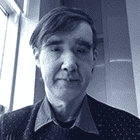
\includegraphics{images/team/team-5.png}
\end{wrapfigure}

Eugene是Stegos网站可靠性工程师,负责我们的开发和生产架构。Eugene在DevOps/SRE有超过30年的经验,从著名的俄罗斯科学院西伯利亚分院在互联网的早期就开始了。他协助搭建并且管理和不同行业的网络和运营架构,包括科学、电信、媒体和金融等。他在很多知名公司都是高级DevOps/SRE职位,并且将这些技术带入了Stegos,确保了整体网络最高的安全性和高效性。

通过Eugene的社交网络,可以找到更多信息。 \href{https://www.linkedin.com/in/eugenechupriyanov/}{LinkedIn profile}.
}

\section{Volodymyr Motylenko, 软件工程师}

{
\setlength\intextsep{0pt}
\begin{wrapfigure}{l}{0pt}
	
\includegraphics{images/team/team-6.png}
\end{wrapfigure}

Volodymyr很年轻但却是分布式系统、加密学和区块链方面的专家。他的硕士论文专注于设计和部署秘钥和密码管理的可信平台模块(TPM)。Volodymyr是领先私有区块链项目的核心团队成员,他贡献了输入/输出层和内部节点网络协议。他加入Stegos,并且会专注于高效算法,同时也有Rust程序语言的实际经验。

通过Volodymyr的社交网络,可以找到更多信息。 \href{https://linkedin.com/in/vldm}{LinkedIn profile}.
}

\chapter{通证经济学}\label{app:token-economics}

\todo[inline]{Fix the partner images}
\comment{
\newcommand{\imgscale}{0.3}
\begin{multicols}{7}[\columnsep=1cm]
	
\includegraphics[scale=\imgscale]{images/partners/partners-1.png}
	\columnbreak
	
\includegraphics[scale=\imgscale]{images/partners/partners-2.png}
	\columnbreak
	
\includegraphics[scale=\imgscale]{images/partners/partners-3.png}
	\columnbreak
	
\includegraphics[scale=\imgscale]{images/partners/partners-4.png}
	\columnbreak
	
\includegraphics[scale=\imgscale]{images/partners/partners-5.png}
	\columnbreak
	
\includegraphics[scale=\imgscale]{images/partners/partners-6.png}
	\columnbreak
	
\includegraphics[scale=\imgscale]{images/partners/partners-7.png}
\end{multicols}
}

\section{融资目标}
Stegos将要共发行10亿STG代币,其中51.25\%将进行公开售卖,从而融资2000万美金,剩余的48.75\% 会用于支付给团队成员、投资人以及顾问等,下个章节会有详细的信息。这些数值都是经过非常仔细的选择,从而让我们可以完成开发的目标,并且启动Stegos生态系统。

Stegos会在所有融资以及资金使用阶段都会有严格的KYC/AML流程,资金主要的用途:

\begin{itemize}
	\item 通过教育项目扩大Stegos生态系统
	\item team打造世界级别的研发 (R\&D)
	\item 急速区块链在不同市场和企业的应用
	\item 推动开发并且吸引最好的人才
\end{itemize}

Stegos的愿景是雄心勃勃的,有着同样雄心勃勃的目标!

\section{代币分配}

\begin{figure}[h!]
\centering
		
\resizebox{.8\textwidth}{!}{%
	
\def\angle{0}
\def\radius{3}

\definecolor{aqua}{rgb}{0.0, 1.0, 1.0}
\definecolor{applegreen}{rgb}{0.55, 0.71, 0.0}
\definecolor{ao(english)}{rgb}{0.0, 0.5, 0.0}

\def\cyclelist{{"green","blue","red","yellow","aqua","orange"}}
\newcount\cyclecount \cyclecount=-1
\newcount\ind \ind=-1
\begin{tikzpicture}[nodes = {font=\sffamily}]
\foreach \percent/\name in {
	51.25/公开销售,
	16.75/技术开发,
	10.0/市场 \& 生态系统,
	10.0/预留,
	10.0/团队,
	2.0/顾问 \& 核心支持者
} {
	\ifx\percent\empty\else               % If \percent is empty, do nothing
	\global\advance\cyclecount by 1     % Advance cyclecount
	\global\advance\ind by 1            % Advance list index
	\ifnum6<\cyclecount                 % If cyclecount is larger than list
	\global\cyclecount=0              %   reset cyclecount and
	\global\ind=0                     %   reset list index
	\fi
	\pgfmathparse{\cyclelist[\the\ind]} % Get color from cycle list
	\edef\color{\pgfmathresult}         %   and store as \color
	% Draw angle and set labels
	\draw[fill={\color!50},draw={\color}] (0,0) -- (\angle:\radius)
	arc (\angle:\angle+\percent*3.6:\radius) -- cycle;
	\node at (\angle+0.5*\percent*3.6:0.7*\radius) {\percent\,\%};
	\node[pin=\angle+0.5*\percent*3.6:\name]
	at (\angle+0.5*\percent*3.6:\radius) {};
	\pgfmathparse{\angle+\percent*3.6}  % Advance angle
	\xdef\angle{\pgfmathresult}         %   and store in \angle
	\fi
};
\end{tikzpicture}
}%
\bigskip

% \caption{Token allocation}
\label{fig:token-allocation}
\end{figure}

\begin{table}[ht!]
\centering
\begin{tabular}{@{\extracolsep{4pt}}ll}
	\toprule[2pt] 比例 & 目标 \\ 
	\midrule[2pt]
	51.25\% & 公开销售 \\
	16.75\% & 技术开发 \\
	10\% & 市场 \& 生态系统 \\
	10\% & 预留 \\
	10\% & 团队 \\
	2\% & 顾问以及核心支持者 \\
	\bottomrule[2pt]
\end{tabular}
\caption{Token allocation} 
\end{table}

\section{代币发行}
STG代币释放会从在前4年以初始代币的14\% 开始,然后每4年进行减半。全新创建的代币会用于区块奖励以及验证节点的服务奖励 (Section \ref{sec:service-award})。

\section{代币销售}

\pgfkeys{
	/pgf/fpu, 
	/pgf/fpu/output format=fixed
}

\newcommand{\setvar}[2] {
	\edef#1{0}
	\FPeval#1{#2}
%	\pgfmathparse{#2}
%	\edef#1{\pgfmathresult}
}

\def\InitialSupply{1000000000} % 1 billion 
\def\PctTokensForSale{51.25} % pct

% Tokens for sale
\setvar\TokensForSale{\InitialSupply * \PctTokensForSale / 100.0}

%%% Existing sales %%% 

\def\SeedPrice{0.013333}
\def\ROnePrice{0.07}
\def\RTwoPrice{0.10}

\def\SeedAmt{1995000}
\def\ROneAmt{9816428.85}
\def\RTwoAmt{4042148.39}

% Total raised
\setvar\SoldAmt{\SeedAmt + \ROneAmt + \RTwoAmt}
% Seed allocation
\setvar\SeedAlloc{\SeedAmt / \SeedPrice / \InitialSupply}
% Round 1 allocation
\setvar\ROneAlloc{\ROneAmt / \ROnePrice / \InitialSupply}
% Round 2 allocation
\setvar\RTwoAlloc{\RTwoAmt / \RTwoPrice / \InitialSupply}
% Sold allocation
\setvar\SoldAlloc{\SeedAlloc + \ROneAlloc + \RTwoAlloc}

% Seed tokens
\setvar\SeedTokens{\SeedAmt / \SeedPrice}
% Round 1 tokens
\setvar\ROneTokens{\ROneAmt / \ROnePrice}

% Round 2 tokens
\setvar\RTwoTokens{\RTwoAmt / \RTwoPrice}
% Total tokens
\setvar\SoldTokens{\SeedTokens + \ROneTokens + \RTwoTokens}
% Seed percentage sold
\setvar\SeedPctSold{\SeedTokens / \TokensForSale}
% Round 1 percentage sold
\setvar\ROnePctSold{\ROneTokens / \TokensForSale}
% Round 2 percentage for sale
\setvar\RTwoPctSold{\RTwoTokens / \TokensForSale}
% Total percentage for sale
\setvar\TotalPctSold{\SeedPctSold + \ROnePctSold + \RTwoPctSold}

%%% Future sales %%% 

\def\ExchOnePrice{0.023}
\def\ExchTwoPrice{0.033}

\def\ExchOneAlloc{0.09}
\def\ExchTwoAlloc{0.0922}

% Exchange allocation 
\setvar\ExchAlloc{\ExchOneAlloc + \ExchTwoAlloc}
% Stage 1 tokens
\setvar\ExchOneTokens{\ExchOneAlloc * \InitialSupply}
% Stage 2 tokens
\setvar\ExchTwoTokens{\ExchTwoAlloc * \InitialSupply}
% Tokens sold 
\setvar\ExchTokens{\ExchOneTokens + \ExchTwoTokens}
% Stage 1 amount
\setvar\ExchOneAmt{\ExchOneTokens * \ExchOnePrice}
% Stage 2 amount
\setvar\ExchTwoAmt{\ExchTwoTokens * \ExchTwoPrice}
% Total sold
\setvar\ExchAmt{\ExchOneAmt + \ExchTwoAmt}
% Stage 1 percentage for sale
\setvar\ExchOnePctSale{\ExchOneTokens / \TokensForSale}
% Stage 2 percentage for sale
\setvar\ExchTwoPctSale{\ExchTwoTokens / \TokensForSale}
% Total percentage for sale
\setvar\ExchPctSale{\ExchOnePctSale + \ExchTwoPctSale}

%%% Global totals

% Tokens
\setvar\TotalTokens{\SoldTokens + \ExchTokens}
% Amount
\setvar\TotalAmt{\SoldAmt + \ExchAmt}
% Allocation
\setvar\TotalAlloc{\SoldAlloc + \ExchAlloc}
% Percentage for sale
\setvar\TotalPctSale{\TotalPctSold + \ExchPctSale}
% Seed percentage of raise
\setvar\SeedPctRaise{\SeedAmt / \TotalAmt}
% Round 1 percentage of raise
\setvar\ROnePctRaise{\ROneAmt / \TotalAmt}
% Round 2 percentage of raise
\setvar\RTwoPctRaise{\RTwoAmt / \TotalAmt}
% Total percentage of raise
\setvar\TotalPctRaise{\SeedPctRaise + \ROnePctRaise + \RTwoPctRaise}
% Stage 1 percentage of raise
\setvar\ExchOnePctRaise{\ExchOneAmt / \TotalAmt}
% Stage 2 percentage of raise
\setvar\ExchTwoPctRaise{\ExchTwoAmt / \TotalAmt}
% Total percentage of raise
\setvar\ExchPctRaise{\ExchOnePctRaise + \ExchTwoPctRaise}
% Total percentage of raise
\setvar\PctRaise{\TotalPctRaise + \ExchPctRaise}

\pgfkeys{/pgf/fpu=false}

\pgfkeys{
	/NoDC/.style={
		/pgf/number format/.cd,% <- changes the prefix for the following options
		fixed,
		%use comma,
		fixed zerofill,
		precision=0,
		1000 sep={,},
	},
	/TwoDC/.style={
		/pgf/number format/.cd,% <- changes the prefix for the following options
		fixed,
		%use comma,
		fixed zerofill,
		precision=2,
		1000 sep={,},
	},
	/ThreeDC/.style={
		/pgf/number format/.cd,% <- changes the prefix for the following options
		fixed,
		%use comma,
		fixed zerofill,
		precision=3,
		1000 sep={,},
	},
}

\newcommand{\pAmt}[1] {
	\pgfmathprintnumber[/NoDC]{#1}
}

\newcommand{\pPct}[1] {
	\pgfmathparse{#1 * 100}
	\pgfmathprintnumber[/TwoDC]{\pgfmathresult}\%
}

\newcommand{\pPrice}[1] {
	\$\pgfmathprintnumber[/ThreeDC]{#1}
}

以前和未来的代币销售:
\bigskip

\begin{table}[htp!]
\centering
\begin{tabular}{@{\extracolsep{4pt}}lllllll}
	\toprule[1pt] 
	{} & \multicolumn{6}{c}{已完成代币销售} \\
	\cmidrule{2-7}
	轮次 & 代币数量 & 价格 & \% 代币 & \% for 销售 & 数量 & \% 融资 \\
	\midrule[1pt]
	种子轮 & \pAmt{\SeedTokens} & \pPrice{\SeedPrice} & \pPct{\SeedAlloc} & \pPct{\SeedPctSold} & \$\pAmt{\SeedAmt} & \pPct{\SeedPctRaise} \\
	第一轮 & \pAmt{\ROneTokens} & \pPrice{\ROnePrice} & \pPct{\ROneAlloc} & \pPct{\ROnePctSold} & \$\pAmt{\ROneAmt} & \pPct{\ROnePctRaise} \\
	第二轮 & \pAmt{\RTwoTokens} & \pPrice{\RTwoPrice} & \pPct{\RTwoAlloc} & \pPct{\RTwoPctSold} & \$\pAmt{\RTwoAmt} & \pPct{\RTwoPctRaise} \\
	\bottomrule[1pt]
	Total & \pAmt{\SoldTokens} & {} & \pPct{\SoldAlloc} & \pPct{\TotalPctSold} & \$\pAmt{\SoldAmt} & \pPct{\TotalPctRaise} \\
	\toprule[1pt] 
	{} & \multicolumn{6}{c}{计划代币销售} \\
	\cmidrule{2-7}
	轮次 & 代币数量 & 价格 & \% 代币 & \% for 销售 & 数量 & \% 融资 \\
	\midrule[1pt]
	第一轮 & \pAmt{\ExchOneTokens} & \pPrice{\ExchOnePrice} & \pPct{\ExchOneAlloc} & \pPct{\ExchOnePctSale} & \$\pAmt{\ExchOneAmt} & \pPct{\ExchOnePctRaise} \\
	第二轮 & \pAmt{\ExchTwoTokens} & \pPrice{\ExchTwoPrice} & \pPct{\ExchTwoAlloc} & \pPct{\ExchTwoPctSale} & \$\pAmt{\ExchTwoAmt} & \pPct{\ExchTwoPctRaise} \\
	\bottomrule[1pt]
	共计 & \pAmt{\ExchTokens} & {} & \pPct{\ExchAlloc} & \pPct{\ExchPctSale} & \$\pAmt{\ExchAmt} & \pPct{\ExchPctRaise} \\
	\addlinespace
	\toprule[2pt] 
	\midrule[0pt]
	整体共计 & \bm{\mathbf{\pAmt{\TotalTokens}}} & {} & \bm{\mathbf{\pPct{\TotalAlloc}}} & \bm{\mathbf{\pPct{\TotalPctSale}}} & \bm{\mathbf{\$\pAmt{\TotalAmt}}} & \bm{\mathbf{\pPct{\PctRaise}}} \\
	\bottomrule[2pt]
	
\end{tabular}
\caption{代币销售} 
\end{table}

\newpage
\section{代币锁仓和释放}

私募轮购买的代币会有锁仓和释放的计划,这部分代币会在主网上线后根据以下计划逐步释放:

\bigskip

\begin{table}[ht]
\centering
\begin{tabular}{lccccccccccc}
	\toprule[2pt] 
	{} & \multicolumn{11}{c}{主网上线后的月份} \\
	\cmidrule{2-12}
	{} & 1 & 2 & 3 & 4 & 5 & 6 & 7 & 8 & 9 & 10 & 11 \\
	\midrule[2pt]
	种子轮 & {} & {} & {} & 12.5\% & 12.5\% & 12.5\% & 12.5\% & 12.5\% & 12.5\% & 12.5\% & 12.5\% \\
	第一轮 & 50\% & 10\% & 10\% & 10\% & 10\% & 10\% & {} & {} & {} & {} & {} \\
	第二轮 & 70\% & 10\% & 10\% & 10\% & {} & {} & {} & {} & {} & {} & {} \\
	\bottomrule[2pt]
\end{tabular}
\caption{解锁细则} 
\end{table}

团队代币的50\% 会从主网上线时锁仓12个月,其余的可能会根据公司的资金需求进行小批量售卖。

锁定的代币无法转移,但是可以用于权益抵押。

\comment{
\chapter{Partners}

\newcommand{\pic}[1]{
	\framebox{
		\includegraphics[clip]{images/partners/#1.png}
	}
}

\newcolumntype{i}{
	@{\hspace{1ex}}
	>{\collectcell\pic}
	c<{\endcollectcell}
}

\begin{table}[ht] 
\centering	
\begin{tabular}{iii}
	partners-1 & partners-2 & partners-3 \\
	partners-4 & partners-5 & partners-6 \\
	empty & partners-7 & empty \\
\end{tabular}
\end{table}
}

\chapter{法律声明}

白皮书没有任何部分构成法律、商业或者税收建议,请在进行任何操作之前,咨询自己的法律、金融、税务或者其他专业人士。Stegos AG (“Stegos”)以及附属机构,Stegos团队成员不为任何通过Stegos发布的白皮书或者其他材料,直接或者间接的损害、损失或者债务负责。

对于Stegos白皮书的英文版本没有任何官网的翻译版本,任何其他语言的翻译请格外注意,因为其中的信息可能会和此白皮书有冲突。

通过访问本白皮书或其任何部分,您向Stegos、其关联公司和Stegos团队声明并保证,您承认、理解并同意:

\begin{enumerate}[label=(\alph*)]
	\item 本文中指的STG代币(“代币”)并没有任何价值,并且也不保证其未来的价值和流动性,并且此代币并非是投机;
	
	\item Stegos以及其附属公司,Stegos团队成员不会为代币价值,代币的转移以及流动性,以及任何第三方代币销售负责;
	
	\item 对于代币购买的任何决定,你不会依赖于此白皮书中的任何声明;
	
	\item 你自己需要确认符合法律、监管要求以及任何法律限制;
	
	\item 这里的信息只适用于瑞士法律,并且管辖地为瑞士楚格;
	
	\item Stegos以及其附属公司,以及Stegos团队,可能会因为未来的法律问题,代币销售活动(TGE)或者其他类似活动可能会被限制,因此可能会通过除了Stegos以外的合法机构发行代币。
	
	\item Stegos以及其附属公司,以及Stegos团队可能会被禁止进行代币销售或者在二级市场进行售卖,也可能会因为法律原因无法在某些交易平台进行交易。

	\item 如果你所在国家将代币销售认为是证券销售,那么你也许无法获得任何代币,也可能会因为你当地的法律而无法参与代币销售,Stegos平台也可能会因此禁止销售代币。
	
\end{enumerate}

本白皮书不得解释为邀请或招揽在任何司法管辖区进行投资或参与证券(无论名称如何)或投资产品的销售。本白皮书中的信息仅供一般说明和讨论之用,Stegos对本信息的准确性和完整性不作任何保证。Stegos保留自行决定更改此处所含信息的权利。本白皮书所载信息对Stegos及其附属公司和Stegos团队成员不具有法律约束力。代币的任何发行或分配协议应由一份单独的协议管辖,该协议规定了相关条款和条件。如果此类协议与本白皮书之间存在任何不一致之处,应以协议的条款和条件为准。

\newpage \appendix
\addtocontents{toc}{\protect\setcounter{tocdepth}{0}}
\addappheadtotoc

\chapter{交易和转账}

\section{UTXO}
为了便于说明,假设Alice向Bob转账代币。Alice的公钥是$P_A$,Bob的秘钥是$s_B$,而且他的公钥是$P_B$。为了保证匿名性,Stegos里的公钥是都是从很大的有限数中选取的随机数,$Z_r$。

当Alice向Bob转账,她会通过Pedersen承诺把数字隐藏,这是绑定且隐藏的。它会将Alice和她的承诺绑定,从而让她无法改变代币的数量。这个承诺也可以向公众隐藏代币数量,也会同步像公众提出证据,表示这个代币的数量是合法的。只有Alice和Bob知道转移了多少代币。

\subsection{Pedersen Commitment 以及Bulletproof} 为了形成Pedersen承诺,Alice将椭圆曲线组$E_r$的主要订单$r$的金额乘以生成器$A$。因此,她可以通过增加公开可知的生成器$G$中的乘数$\gamma$,这个乘数是从有限区域$Z_r$中随机选择,从而掩盖承诺。生成器$A$和$G$必须没有已知的关系。将掩盖系数放入主要的生成器曲线中是非常重要,这也是持有所有公钥的曲线。

因此,Pedersen commitment会变成:
$$ C(x, \gamma) = x \, A + \gamma \, G \in E_r$$
$$x, \gamma \in Z_r,$$

其中$x$ 代表了转移代币的数量,$A$是数量曲线生成器,同时$G$是核心生成器。我们用$C(x, \gamma)$代表这个commitment.

这个commitment的数值会包装在Bulletproof的区间证明$x$, 同时也证明了这个数值是在合理64字符的范围内。

\subsection{目标地址隐藏} Alice然后会通过系数$\delta \in Z_r$去隐藏Bob的公钥,而不是Bob初始的公钥$P_B$,她会输入UTXO $P_{B, \delta} = P_B + \delta \, G$。

\subsection{加密有效载荷} Alice必须要传递$x$的数值,并且向Bob隐藏$\gamma$和$\delta$参数。她可以将这个信息包含到UTXO的\textit{加密有效载荷}。除了上面所说的数值,加密有效载荷也需要包含Alice想要和Bob分享的随机数。

为了生成加密有效载荷,Alice必须要选择随机数$\alpha, k \in Z_r$会用于创建并隐藏对称数据秘钥。
实际的对称秘钥将会是$H(k \, G)$。为了将数据安全地通过区块链传递给Bob,Alice需要通过 $\alpha$ 将其隐藏,并且存储在以下的UTXO中:$$\mathit{Key}_{\alpha} = (\alpha \, P_{B} + k \, G, \alpha \, G )$$。

Alice会使用$H(k \, G)$秘钥,并通过AES-128加密她的有效载荷,同时也会将加密有效载荷放入$E_B(x, \gamma, \delta)$的UTXO。

当Bob收到UTXO后,他会从$\mathit{Key}_{\alpha}$中提取它,并将他的秘钥$s_B$和数组的第二个元素相乘,最终得到$s_B \, \alpha \, G = \alpha \, P_B$,然后减去第一个元素去找到$k \, G$。然后,他可以找到$H(k \, G)$,加上计算对称秘钥,然后解密Alice发给他的有效载荷。

\subsection{TTL以及数据规模} Alice会设置TTL(生存时间)以及UTXO的$Size_{data}$为零,从而显示这里是\textit{monetary UTXO}。

\subsection{UTXO ID} Alice会通过将整个UTXO进行哈希算法,从而形成UTXO $\mathit{ID}$,其中包含了Bob公钥的隐藏版本$P_{B, \delta}$、Pedersen commitment以及Bulletproof、TT、$Size_{data}$以及加密载荷。

UTXO $\mathit{ID}$ 成为了独特的标识符,因此如果所有其他的都是相等的,那么$\gamma$ 和 $\delta$参数就会随机从$Z_r$中选择。

\subsection{UTXO结构}
因此,UTXO的最终结构是如下:

\begin{multline*}
UTXO = (ID, P_{B, \delta}, Bp, TTL, Size_{data},\\
Key_{\alpha}, E_B(x, \gamma, \delta))
\end{multline*}

其中

\begin{align*}
ID &= H(P_{B, \delta}, Bp, TTL, Size_{data}, \\ 
& Key_{\alpha}, E_B(x, \gamma, \delta)) \in Z_r \\
H(arg_1, arg_2, ...) &= \textit{hash mapping of concat args} \\
P_{B, \delta} &= P_B + \delta \, G \\
G &= \textit{known generator for group } E_r \\
Bp &= \textit{Bulletproof and Pedersen} \\
& \textit{commitment on amount}, x 
\end{align*}

\begin{align*}
TTL &= \textit{Time-to-Live}, 0 \\
Side_{data} &= \textit{Data payload size}, 0 \\
Key_{\alpha} &= (\alpha \, P_{B} + k \, G, \alpha \, G ) \\
E_B(x, \gamma, \delta) &= \textit{AES-128 encrypted payload}
\end{align*}

Alice和Bob的公钥都不会在任何地方显示。我们只会展示Bob公钥的隐藏版,而且由于$\delta$的数值是加密的,没人可以通过这个数值获得真正的公钥。

因此,Bob可以在自己的网站或者发票上公开自己的公钥,而不用担心自己的身份会被查询到,因为他的公钥在Stegos的UTXO里面总是隐藏的,并且是以全新且随机的数字。

\section{交易转账架构}
当Bob想要花费他的新代币时,他必须要形成包含输入(TXINs)和输出(TXOUTs)的列表。TXINs是对应其他UTXO的$\mathit{ID}$s,而TXOUTs是全新UTXO的列表。他也必须要在整个交易中提供有效签名,这也同时证明了他对于所有TXINs的拥有权,证明了交易中承载了TXINs、TXOUTs和手续费间的资金净余额为零,并且防止了MITM攻击者。

UTXO只能整体进行消费,如果它有了多余的数值,那么会产生TXOUT并且返回到他自己,然后创建新的UTXO.Bob必须要展示其交易中所有输入的整合等于所有输出的总和加手续费。他可以通过Pedersen commitments完成这个算法,从而让所有的交易数据都和他整合,但是也不会有任何实际的数量泄露。
 
为了完成签名,他会将从代表他UTXO的特定TXINs列表$\mathit{ID}$s中所有$\delta$的隐藏系数都加起来,并且还会加上从Pedersen commitments所有的$\gamma$ 隐藏系数,其是从相同UTXO中的Bulletproofs获得的,同时减去他自己TXOUT UTXOs中的隐藏系数$\gamma$。

假设Bob使用了$N$ TXINs,而且他自己的公钥$P_B = s_B \, G$。那么,他的有效秘钥签名就成为了:
$$s_{\mathit{eff}} = N \, s_B + \sum_{i \in \text{ins}} {\delta_i} + \sum_{i \in \text{ins}}{\gamma_i} - \sum_{j \in \text{outs}}{ \gamma_j}$$

使用这个有效秘钥,在随机选择$k \in Z_r$,他会产生Schnorr签名交易对$(u, K)$:
$$K = k \, G$$
$$u = k + H_r(K, P_{eff}, H(T)) \, s_{\mathit{eff}}$$
$$Sig(s_{eff},T) = (u, K)$$
so that validators can see that:
$$u \, G = K + H_r(K, P_{eff}, H(T)) \, P_{eff}$$
$$P_{\mathit{eff}} = \sum_{i \in \text{ins}}{P_i} + \sum_{i \in \text{ins}}{C_i} - \sum_{j \in \text{outs}}{C_j} - \mathit{Fee} \, A$$
其中$T$代表了整个交易记录,扫描签名。$H_r(x)$ 函数代表了将$H(x)$哈希映射到$Z_r$领域。

让我们检查下这些条件。Pedersen的commitments是叠加同态的:
$$C(x_1, \gamma_1) + C(x_2, \gamma_2) = C(x_1 + x_2, \gamma_1 + \gamma_2)$$

因此,如果Bob的交易是有效的,在 $\mathit{Fee}$操作后,有效公钥的数字在$A$ 曲线上显示为零余额,剩下的都是在$G$曲线。验证节点综合成为了$G$曲线上另外的公钥,这和他自己的有效秘钥$s_{\mathit{eff}}$完全符合。只有Bob可以获得有效的签名,因为它依赖于他的秘钥,这是无法忘记的。Alice和Bob都知道其他所有秘密的条款,$\gamma$s 和 $\delta$s。没有其他人知道任何秘密数值。

假设Bob现在想把从Alice处拿到的代币在扣除手续费后转移给Charlie。为了这样做,Bob形成了使用不同的UTXO系数$\gamma_2$,以及不同的秘钥隐藏数值$\delta_2$,其中包含了$(x - \mathit{Fee})$。Bob必须要形成全新的Bulletproof,同时也会将这些数值进行加密,而且只有Charlie可以看到:

\begin{multline*}
ID’ = H(P_{S, \delta_2}, Bp’, TTL, Size_{data}, \\
Key_{\alpha_2}, E_S(x - Fee, \gamma_2, \delta_2))
\end{multline*}

其中 $P_{C, \delta_2}$ 是Charlie的隐藏公钥,$TTL$ 和 $Size_{data}$是零,同时$Key_{\alpha_2}$ 是隐藏的对称秘钥。

Charlie能够通过提供一个\textit{ID’}的有效交易签名来花费这个UTXO,就好像Bob对自己输入数据那么做。

Bob的TXOUT现在看起来如下:

\begin{multline*}
\text{TXOUT} = (ID’, P_{S, \delta_2}, Bp’, TTL, Size_{data},\\ 
Key_{\alpha_2}, E_S(x - Fee, \gamma_2, \delta_2))
\end{multline*}

总地来说,Bob发布了如下的交易:

\begin{align*}
\text{T} = \{&\text{TXIN} : \{\mathit{ID}\}, \\
&\text{TXOUT} : \{(ID’, P_{S, \delta_2}, Bp’, TTL, Size_{data}, \\
& \ \ \ \ \ \ \ \ \ \ \ \ \ \ Key_{\alpha_2}, E_S(x - Fee, \gamma_2, \delta_2))\}, \\
&\text{FEE} : \mathit{Fee}, \\
&\text{GAMMA} : \gamma_{\mathit{adj}} = \sum_{i \in \text{ins}}{\gamma_i} - \sum_{j \in \text{outs}}{\gamma_j}\\
&\text{SIG} : \mathit{Sig}(s_B, T)\}
\end{align*}

Bob的TXIN首行代表了Alice的UTXO,第二行是TXOUT,这是Charlie的全新UTXO。第三行显示了这个交易手续费,并且是纯文本格式。

第四行显示了在$G$曲线上的$\gamma$数值,其中面试了整体输入总和等于输出总和,最终TXINs和TXOUTs以及手续费的净余额为零。而且,在交易进入区块链的时候,这个条件会加入到区块总和,从而显示整个区块,会包含很多UTXO,并且继续显示为零余额。

最后一行是Bob的签名,其中表示了整个交易的拥有权,这是基于所有TXIN、TXOUT、手续费以及$\gamma_{adj}$的哈希值。最终的签名也会对交易内容突变作出检查。如果任何东西在记录中改变,那么签名就不会进行检查。因此,Stegos交易是不可改变的。

\chapter{雪球}\label{app:snowball}

\section{形成发送者池}
除了选择全新的见证人和领导者的每个epoch,所有验证节点会在其中选择节点,它们必须要在ValueShuffle协议中作为\textit{Bulletin Board},而且需要将这个节点的公钥包含在全新epoch的密封keyblock。我们将Bulletin Board节点称之为\textit{facilitator}。

每个申请交易的节点应该广播\textit{交易意图}信息,同时还有全新的公钥以及有效性签名认证。

\textit{Facilitators} 应该听取节点的交易意图信息以及每个$K$秘钥的公钥。$K$通过定义应该有多少参与者组成一个交易混合池来定义匿名集的基数。这是一个可调参数,可以为区块链的每个epoch的设置。

在收集$K$密钥或超时$T$秒时,\textit{facilitator}会广播一条\textit{交易池}消息(用其私钥签名),其中包含所有收集到的临时公钥和相应的签名。

每个能够识别\textit{交易池}消息的秘钥都应该进行排序,形成信息收集的哈希,然后使用这个哈希作为\textit{合并交易会话}的随机种子。

\textit{交易池领导}由参与节点通过使用每个池参与者的公钥形成上面定义的哈希值的XOR来选择,如果结果值是列表中的最小值,则该节点应选择为\textit{交易池领导}。

\textit{交易池领导}负责最终交易的发布,我们称为\textit{超级转账}。

\section{建立合并交易部分}
所有交易池部分的通信,包括广播,都 应该包含所有参与者,其中所有节点都会广播他们的TXIN列表,同时还有签名去认证他们是TXIN的所有权。每个参与者都能通过验证签名来对列表进行认证,参与者应该对每个人的TXIN $ID$进行验证,确保公钥和其相匹配。

\subsection{整合输入数据} 
一个参与者在txins上的有效签名是通过在txins中引用的utxos中显示的隐藏公钥的总和上创建schnorr签名形成的:

\begin{align*}
TXIN &= \{ID_1, ID_2, ..., ID_N\}\\
Sig &= (u, K)\\
K &= k \, G \\
s_{cmp} &= N s + \sum_i{\delta_i}\\
P_{cmp} &= N P + (\sum_i{\delta_i})\, G = s_{cmp} \, G\\
u &= k + H_r(K, P_{cmp}, H(ID_1, ID_2, ..., ID_N)) \, s_{cmp},
\end{align*}

其中sum是超过了TXIN的列表,$s$是拥有者的秘钥,$P = s \, G$ 是对应公钥,而且$\delta_i$是公钥隐藏参数。$N$是列表中TXIN的数量,$k$的数值会从$Z_r$中随机选出。

通过以下方式,签名验证会完成:
$$u \, G = K + H_r(K, \sum_i{P_i}, H(ID_1, ID_2, ..., ID_N)) \, \sum_i{P_i}$$
其中$P_i$ 是隐藏的公钥,并且和每个$ID_i$对应,这个签名保证了显示UTXO所对应TXIN的所有权。

此广播中的任何内容都不能识别发件人,但不能指望保持该状态。在错误行为的情况下,一个指责周期将要求每个节点提交其所有共享的秘密密钥,这将有效地揭示它们的完整事务。重新启动将计算新的TXOUT,这样成功的运行将确保参与者的匿名性。但是如果一个怪罪循环被执行,就没有办法再掩盖与TXIN的关联。

一旦从每个参与者那里收到了贡献,或者发生了超时,所有参与者都知道最终的txin池。由于这些仅仅是指向不可变区块链的UTXO$ID$s,因此除了删除单个TXIN引用之外,此列表不会发生进一步的更改,因为在协议期间发现一些参与者脱机,或者当检测到作弊者并随后排除以重新启动协议时。

\subsection{建立成对共享秘钥} 
所有参与者将在他们自己和集合交易会话的每个其他参与者之间建立成对的共享密钥。这些共享密钥用于在匿名协议中形成隐藏因素,这样,只有在汇集所有参与者的结果之后,他们之间共享的数据收集才会变得明显。在那之前,所有的信息都是隐藏的。在此之后,将知道数据,但无法推断出谁提供了数据的哪些部分。

为了使协议工作,在交互时,成对的用户必须始终使用相同的共享秘密隐藏密钥。只有这样,来自所有参与者的所有隐藏因子的总和才会在骰子混合数组中取消。但是用户不能看到彼此的秘密,因为总隐身因素也包括与所有其他参与者相关的贡献,而这些密钥对另一方来说是未知的。

分享的秘钥会通过Diffie-Hellman安全秘钥交换\cite{c21}的方式在每对参与者间秘密建立,并且这可以通过让$A$转账给$B$来完成建立。 
$$A \rightarrow B: (\alpha \, P_B, Sig(P_A))$$
$A$随机选择了$\alpha$,并且其中$Sig(P_A)$安全地验证了这个信息是从$A$获得。这个签名包含了公钥,$P_A$。

然后,$B$会回应$A$:
$$B \rightarrow A: (\beta \, P_A, Sig(P_B))$$
$\beta$ 会从 $B$ 中随机选择。

交换过后,分享的秘钥是产品的哈希值:
$$key = H(\alpha \beta \, G)$$ 

但是由于双方都不知道系数,我们可以在$A$处进行计算:
$$\beta \, G = (\beta \, P_A) / s_A$$
因为 $P_A = s_A \, G$. 而且在$B$处我们计算:
$$\alpha \, G = (\alpha \, P_B) / s_B$$
然后,每方都会将他们选择的随机数乘以结果,从而得到$(\alpha \beta \, G)$。没人可以看到交换过程,这样会避免秘钥分享。

\subsection{为输出数据生成DiceMix排列} 
接下来,每个参与者用\textit{全新的随机数},为最终的集体schnorr签名选择随机的$k$因子,并生成包含碎片txout的dicemix数组,并隐藏其$\gamma_{adj}$和$K$签名值的运行总和。此信息的散列承诺将被签署并广播给所有参与者。此承诺将用于在以下传递过程中验证信息,以验证信息是否正确传输。

DiceMix数组包含TxOut片段的连续幂次,在所有参与者汇集下一次传递的结果后,用自取消种子隐藏。在形成骰子混合数组并运行和之后,这些信息被签名并广播给所有参与者。由于DiceMix密码混合过程,匿名性得到了保证。即使所有参与者都能从附带的签名中看到谁传递了一个骰子混合数组,他们也看不到集合中的哪些组件是由任何给定的参与者贡献的。只有当所有参与者的骰子组合数组相加后,才会显示整个集合。

每个参与者的每个$K$签名项都是一个盲和。我们这样做是为了防止组合探索,一旦签名$U$值被公开,这可能导致TXINS和TXOUT之间的关联。

\subsection{形成超级转账} 
在收到所有骰子组合数组和运行总和后,每个参与者可以使用牛顿恒等式形成多项式,其根是单个贡献。求解多项式的根可以揭示参与者的txout的每个分量。重新组合这些txout,形成一个\textit{超级转账},其中包含显示零余额所需的所有TXIN、TXOUT、$\gamma_{adj}$和一个集合schnorr签名所需的$K$签名和。

每个参与者通过检查$gamma$和的零余额,并验证TXOUT项目符号证明,来验证整个交易的正确性。他们还必须在TXIN和TXOUT列表中找到自己的贡献。如果超级交易没有正确验证,那么就有人作弊了,我们输入一个\textit{错误发现周期}。否则,我们就开始形成集体签名。

\subsection{形成共有Schnorr签名} 
知道超级交易和集体$K_{sum}$ 签名条件后,每个参与者广播其$u$签名组件,与其他参与者的组件相加,从而在整个超级交易上生成集体Schnorr签名。

每个参与者的超级交易中的签名形成都是如下完成:

\begin{align*}
T &= \text{super-transaction} \\
Sig_i &= (u_i, K_{sum}) \\
K_{sum} &= \sum_i{k_i \, G} \\
s_{cmp,i} &= N \, s_i + \sum_{j \in \text{ins}} {\delta_j} + \sum_{j \in \text{ins}} {\gamma_j} - \sum_{k \in \text{outs}} {\gamma_k} \\
P_{cmp,i} &= s_{cmp,i} \, G \\
P_{sum} &= \sum_i{P_{cmp,i}}\\
u_i &= k_i + H_r(K_{sum} , P_{sum},  H(T)) \,  s_{cmp,i}\\
\end{align*}

其中,索引$i$标记每个参与者,索引$j$标记每个TXIn,其中$N$标记属于参与者,索引$k$标记属于该参与者的每个TXOUT。所有参与者汇总后,多签名$(u_{sum}, K_{sum})$表示超级交易上的有效签名,其方式与如果这是简单交易时的方式相同。

\subsection{发布超级转账} 
在这个最后的签名通行证结束时,每个参与者都应该有一个超级交易,可以由公共证人验证。但是TXIN和TXOUT之间的所有连接都将断开。任何人都能看到的是,所有的TXIN都被消耗掉了,每个TXOUT必须从这些TXIN中的一个或多个派生出来,但是没有办法知道哪些是相关联的。\textit{这部分的领先者} 会话负责人,然后使用八卦协议将超级交易发送到网络中进行验证并包含到块中。

\subsection{blame循环} 
如果一定要发生blame循环,每个参与者必须泄露他们共享的秘密密钥。然后,根据先前发送的信息,所有其他节点都可以验证计算的所有阶段是否正确执行。然后我们知道TXIN和TXOUT之间的关联。任何不能或不会这样做的参与者都会被归咎于故障,并且协议会在记录与欺骗节点相关联的TXIN后重新启动。

但是,由于秘密共享密钥在发现过失时被泄露,所有参与者必须从建立新的共享密钥的角度重新启动协议。

\chapter{隐私币综述}\label{app:privacy-coins}

在这一章中,我们简要介绍了最突出的隐私硬币,并分析了它们的隐私保护和性能特点。

\section{隐私币比较}

\begin{table}[ht!]
\centering
\begin{tabular}{llllllllll}
	\toprule[2pt] 
	{} & Unlink\textsuperscript{1}
	& Untrac\textsuperscript{2} & Conf \textsuperscript{3} & Prun\textsuperscript{4} & Shard\textsuperscript{5} & Inter \textsuperscript{6} & Cons\textsuperscript{7} & Trust\textsuperscript{8} & Apps \textsuperscript{9} \\
	\midrule[2pt]
	Monero & Yes & Yes & Yes & No & No & No & PoW & No & No \\
	Zcash  & Yes & Yes & Yes & No  & No & No & PoW & Yes & No \\
	Dash   & No  & Yes & No  & No  & No & No & PoW/PoS & No & No \\
	Grin   & Yes & No  & Yes & Yes & No & Yes & PoW & No & No \\
	Stegos & Yes & Yes & Yes & Yes & Yes & No & PoS & No  & Yes \\
	\bottomrule[2pt]
\end{tabular}
\caption{隐私币的特性} 
\end{table}

\begin{enumerate}
	\item 非链接性。 对于任何2个输出的交易,不可能证明它们转向了同一个人\cite{c2}。
	\item 不可追踪性。对于任何进入的转账,所有可能的发出者都是等概率的\cite{c2}。
	\item 隐私性。通过分析区块链数据进行保护(例如,交易细节等)。  	
	\item 修剪。发出的代币可以通过区块链进行修剪,并且区块链可以压缩。
	\item 分片。可以在参与者或参与者组之间划分的事务验证和块密封过程。
	\item 交互性。交易的发送方和接受者在将交易发布到区块链之前,必须在链外进行交互。
	\item 可信的设置。区块链参与者需要构建信任,从而可以产生初始参数,然后销毁这些参数。
	\item 共识算法
	\begin{enumerate}
		\item PoW。工作量证明,作为比特币的共识协议,其中的节点需要解决很困难的问题(消耗费用和时间),从而可以挖出区块,但是真很容易进行验证。由于计算的复杂性,矿工每年消耗的能源大约是73TWh每年\footnote{https://digiconomist.net/bitcoin-energy-consumption}。
		\item PoS。权益证明是一种共识算法,下个区块的产生是通过不同因素进行随机选择,这些因素包括持有代币的数量、时间以及抵押的资金。PoS区块链对环境更加友好。\footnote{http://cfa-consulting.ch/dlfiles/NxtEnergyandCostEfficiencyAnalysis.pdf}.
	\end{enumerate}
	\item Apps。数据和支付都可以很快速和容易地进行传输,很多应用可以通过交换数据信息而进行沟通。
\end{enumerate}

\section{隐私币描述}

\subsection{门罗币} Monero最初是在2014年以Bitmonero的名义作为一个字节码分支出现的。Monero使用了一个UTXO模型和POW共识,并使用了基于CryptoNote协议\cite{c2}的环签名方法。2017年,Monero实施了RingCT\cite{c3},一个改进版的Ring签名。RINGCT可以对交易的金额和不可追踪性进行保密。结合隐形地址(也在原始的CryptoNote白皮书中介绍),它提供了收件人的不链接性,这提供了完全的隐私和保密性。

Monero的区块链不能被压缩,因为用过的UTXO不能从中删除。永久保存所有的utxo是ringct协议的一个要求,它混淆了事务输入中提到的特定utxo实际上已经被使用的事实。尽管最近推出了Bulletproofs\cite{c4},这取代了Monero最初的零知识范围证明,并将简单的交易规模从13kb减少到2.5kb,但他们不断增长的区块链问题无法解决。


\subsection{大零币} Zcash起源于2016年,作为比特币分叉币,因此使用了UTXO模型和POW共识。Zcash旨在通过关注隐私来修复比特币的缺陷。该项目建立在Zerocoin\cite{c5}上完成的工作基础上,并解决了其中的一些错误,例如证明文件的大小,zcash减少到1KB,加快了验证速度。

为了建立保密性和不可追踪性,Zcash实施了零知识证明 \cite{c6}。为了提供收件人的不链接性,Zcash使用了隐藏地址。

零知识证明可以将匿名性给予所有铸币\footnote{The \textit{匿名集}是在zcash交易中可能是发送者的参与者集,正如一个破坏了一组节点的全局观察者所看到的那样。},这样可以提供很高的隐私性。然而,平均每笔交易的规模高达2千字节,再加上一个不断增长的累加器,它必须保存所有用过的硬币的序列号,因此不能进行删减,这使得zcash的可扩展性大大降低。可伸缩性问题是隐私当前是可选的,而不是默认的主要原因。在写入时,不到25\%的交易被屏蔽。

zk-snarks协议的另一个可疑部分是初始的可信设置。Zcash利用了一个多部分的方式,涉及几个值得信赖的人。这是有争议的,因为用户必须相信所有这些人都破坏了他们的初始参数,并且相信整个方式是正确进行的。

\subsection{达世币} Dash最初是莱特币的一个代码基分叉(因此也是比特币的一个分叉),并于2014年1月作为XCoin推出。Dash使用UTXO模型和POW共识。

除了标准的节点和矿工,Dash有\textit{主节点},这个节点必须要有静态的IP地址,同时也满足CPU、RAM和硬盘空间的需求。每个主节点必须拥有至少1000DASH,服务证明协议可以保证主节点有最多目前的区块链协议,并且保持在线。

需要注意到在Dash中隐私是可选的,并且通过主节点的\textit{InstantSend}功能,Dash可以承载大量的交易。

CoinJoin部署了\textit{PrivateSend}功能,这是由比特币核心开发者Gregory Maxwell\footnote{https://bitcointalk.org/index.php?topic=279249.0}首次提出的不可追踪解决方案。在PrivateSend中,三个用户将他们的代币合成一个大额转账,然后将代币发送至全新生成的地址。因此,这些代币就会在三个参与者间混合,打破了他们之间的所有权轨迹。这个流程可以自动重复8次,并且是根据不同的参与者,这样做可以保证非常高的隐私性。

Dash不会提供InstantSend或者PrivateSend里面的隐私性。而且,CoinJoin协议需要用户的输入数据都有相同金额,这个要求对于隐藏金额来说是不可能的。

作为进一步的隐私漏洞,Dash的用户必须相信主节点在发送交易时会保持用户的IP地址不被公开,并且与用户的UTXO不链接。

\subsection{MimbleWimble} Mimblewimble是一个匿名用户在比特币开发者聊天室中以Tom Elvis Jedusor的名义提出的协议,他在文章\footnote{https://download.wpsoftware.net/bitcoin/wizardry/mimblewimble.txt}上留下了一个链接,概述了一个协议,以显著提高比特币网络的可扩展性和隐私性。

mimblewimble基于Greg Maxwell的机密交易设计思想\footnote{https://people.xiph.org/\texttt{\~}greg/confidential\_values.txt},除了Mimblewimble之外,它的生成用于掩盖交易量的随机盲因子的接收者。然后,这个致盲因素被接收者用作所有权证明,因此同时作为接收者的公钥。因此,Mimblewimble在其交易中为接收者的数量和不可链接性提供了保密性。

Mimblewimble中交易的不可跟踪性建立在来自CoinJoin的思想基础上,通过打破交易边界和只在新挖掘的块中存储矿工验证的所有交易的输入和输出来实现。

Mimblewimble实现使用UTXO模型和POW共识。对于新生成的块的输入中引用的每个UTXO,可以递归地应用一个简单的修剪算法来修剪用过的UTXO。

但是,Mimblewimble中也有几个缺点:

\begin{itemize}
  \item {为了创建交易,发送者和接收者必须首先进行交互。发送方不能将交易过账到区块链,除非先用不完整的交易数据联系接收者,然后等待一个盲目因素的响应。}
  \item {用户必须相信,矿工不会跟踪事务中输入和输出的历史记录,而是在挖掘块后完全丢弃此数据。由于无法保证这一点,对代币的可替换性和使用者的隐私权构成了威胁。}
\end{itemize}


\newpage
\raggedright
% \bibliographystyle{unsrt}
% \bibliography{biblio}

\begin{thebibliography}{99}

\bibitem{c1} Satoshi Nakamoto. ``Bitcoin: A Peer-to-Peer Electronic Cash System,’’ https://bitcoin.org/bitcoin.pdf, October 31, 2008.

\bibitem{c2} Nicolas van Saberhagen. ``CryptoNote v 2.0,’’ https://cryptonote.org/whitepaper.pdf, October 17, 2013.

\bibitem{c3} Shen Noether, Adam Mackenzie and Monero Core Team. ``Ring Confidential Transactions,’’ https://lab.getmonero.org/pubs/MRL-0005.pdf, February, 2016.

\bibitem{c4} Benedikt Buenz, Jonathan Bootle†, Dan Boneh, Andrew Poelstra, Pieter Wuille, and Greg Maxwell. ``Bulletproofs: Short Proofs for Confidential Transactions and More,’’ Cryptology ePrint Archive, Report 2017/1066, 2017. URL: https://eprint.iacr.org/2017/1066.

\bibitem{c5} I. Miers, C. Garman, M. Green and A. D. Rubin. ``Zerocoin: Anonymous Distributed E-Cash from Bitcoin,’’ 2013 IEEE Symposium on Security and Privacy, Berkeley, CA, 2013, pp. 397-411. URL: https://ieeexplore.ieee.org/document/6547123

\bibitem{c6} Nir Bitansky, Ran Canetti, Alessandro Chiesa, and Eran Tromer. 2012. ``From extractable collision resistance to succinct non-interactive arguments of knowledge, and back again,’’ in Proceedings of the 3rd Innovations in Theoretical Computer Science Conference (ITCS ‘12). ACM, New York, NY, USA, 326-349. URL: https://dl.acm.org/citation.cfm?id=2090263

\bibitem{c7} Tim Ruffing and Pedro Moreno-Sanchez. ``Mixing Confidential Transactions: Comprehensive Transaction Privacy for Bitcoin,’’ Cryptology ePrint Archive, Report 2017/238, 2017. URL: https://eprint.iacr.org/2017/238

\bibitem{c8} Torben Pryds Pedersen. ``Non-Interactive and Information-Theoretic Secure Verifiable Secret Sharing,’’ Advances in Cryptology — CRYPTO ‘91”, Springer Berlin Heidelberg, 1992, pages 129–140.

\bibitem{c9} Miguel Castro and Barbara Liskov. ``Practical Byzantine Fault Tolerance,’’ Proceedings of the Third Symposium on Operating Systems Design and Implementation, 1999, pages 173–186. 

\bibitem{c10} Ewa Syta, Iulia Tamas, Dylan Visher, David Isaac Wolinsky, Philipp Jovanovic, Linus Gasser, Nicolas Gailly, Ismail Khoffi, Bryan Ford. ``Keeping Authorities “Honest or Bust” with Decentralized Witness Cosigning,’’ arXiv:1503.08768v4 [cs.CR], 30 May 2016. URL: https://arxiv.org/pdf/1503.08768.pdf

\bibitem{c11} Eleftherios Kokoris-Kogias, Philipp Jovanovic, Nicolas Gailly,
Ismail Khoffi, Linus Gasser, and Bryan Ford. ``Enhancing Bitcoin Security and Performance with Strong Consistency via Collective Signing,’’ arXiv:1602.06997v3 [cs.CR], 1 Aug 2016. URL: https://arxiv.org/pdf/1602.06997v3.pdf

\bibitem{c12} Ewa Syta, Philipp Jovanovic, Eleftherios Kokoris Kogias, Nicolas Gailly, Linus Gasser, Ismail Khoffi, Michael J. Fischer, Bryan Ford. ``Scalable Bias-Resistant Distributed Randomness,’’ Cryptology ePrint Archive, Report 2016/1067, 2016. URL: https://eprint.iacr.org/2016/1067.

\bibitem{c13} Ignacio Cascudo, Bernardo David. ``SCRAPE: Scalable Randomness Attested by Public Entities,’’ Applied Cryptography and Network Security, Springer International Publishing, 2017, pages 537–556.

\bibitem{c14} Youliang Tian, Changgen Peng, Renping Zhang, Yuling Chen. ``A practical publicly verifiable secret sharing scheme based on bilinear pairing,’’ 2nd International Conference on Anti-counterfeiting, Security and Identification, IEEE, 2008.

\bibitem{c15} M. Stadler. ``Publicly verifiable secret sharing,’’ in Advances in Cryptology—EUROCRYPT ’96, volume 1070 of Lecture Notes in Computer Science, pages 190–199, Berlin, 1996. Springer-Verlag.

\bibitem{c16} Dan Boneh, Ben Lynn, Hovav Shacham. ``Short Signatures from the Weil Pairing, ‘’ Journal of Cryptology”, 2004, volume 17, pages 297–319.

\bibitem{c17} Tim Ruffing, Pedro Moreno-Sanchez, Aniket Kate. ``CoinShuffle: Practical Decentralized Coin Mixing for Bitcoin,’’ University of Saarland, Germany, 2014. URL: http://crypsys.mmci.uni-saarland.de/projects/CoinShuffle/coinshuffle.pdf

\bibitem{c18} Tim Ruffing, Pedro Moreno-Sanchez, Aniket Kate. ``P2P Mixing and Unlinkable Bitcoin Transactions,’’ University of Saarland, Germany, 2016. URL: https://crypsys.mmci.uni-saarland.de/projects/FastDC/paper.pdf

\bibitem{c19} Tim Ruffing, Pedro Moreno-Sanchez. ``Mixing Confidential Transactions: Comprehensive Transaction Privacy for Bitcoin,’’ Cryptology ePrint Archive, Report 2017/238, 2017. URL: https://eprint.iacr.org/2017/238

\bibitem{c20} David Chaum. ``The dining cryptographers problem: Unconditional sender and recipient untraceability,’’ Journal of Cryptology”, 1988, volume 1, pages 65–75.

\bibitem{c21} Whitfield Diffie, , Martin E. Hellman. ``New Directions in Cryptography,’’   in IEEE Transactions on Information Theory, volume 22 (6), pages 644–654. 

\bibitem{c22} C.P. Schnorr. ``Efficient Identification and Signatures for Smart Cards,’’
in Advances in Cryptology — CRYPTO’ 89, 1990, Springer, pages 239–252.

\bibitem{c23} Bruno Fran{\c c}a, Marvin Wissfeld, Pascal Berrang, Philipp von Styp-Rekowsky, Reto Trinkler. ``Albatross: An optimistic consensus algorithm,’’ March 2019. URL: https://arxiv.org/abs/1903.01589
	
\end{thebibliography}

\end{CJK*}
\end{document}
